\documentclass[abstracton,12pt]{scrartcl}
    
\usepackage[utf8]{inputenc}
% \usepackage[T1]{fontenc}
\usepackage{fancyhdr}
\usepackage{graphicx}
\usepackage{tikz}
\usepackage{listings}
\usepackage{amssymb}
\usepackage{amsfonts}
\usepackage{amsmath}
\usepackage{amsthm}
\usepackage{pdfpages}
\usepackage{forest}
\usepackage{multicol}
\usepackage{varwidth}
\usepackage{verbatim}
\usepackage{minted}
\usepackage{framed}
\usepackage[ruled,vlined]{algorithm2e}
\usepackage{caption}
\usepackage{subcaption}
\usepackage{cleveref}
\usepackage{soul}
\usepackage{float}
\usepackage{wrapfig}
% \usepackage{geometry}
% \usepackage{titlesec}

% \forestset{qtree/.style={for tree={parent anchor=south, child anchor=north,align=left,inner sep=0pt}}}
\graphicspath{
  {images/},
  {images/1_unprod_nodes/},
  {images/2_unprod_nodes_tau/}
  {images/3_unprod_nodes_L/}
}

% \setlength{\multicolsep}{6.0pt plus 2.0pt minus 1.5pt}% 50% of original values
% \titleformat{\chapter}{}{\thechapter}{}{}
% \titlespacing{\chapter}{-100pt}{-100pt}{-100pt}

% --------- 

\titlehead{Department of Informatics, University of Zürich}
\subject{\vspace*{2cm}BSc Thesis}
\title{An Adaptive Index for Hierarchical Distributed Database Systems}
\author{
    Rafael Kallis\\[-5pt]
    \scriptsize Matrikelnummer: 14-708-887\\[-5pt]
    \scriptsize Email: \texttt{rk@rafaelkallis.com}
}
\date{\vspace*{2cm}February 1, 2018}
\publishers{
    \small supervised by Prof.\ Dr.\ Michael\ Böhlen and Kevin\ Wellenzohn \\[5cm]
    \begin{tikzpicture}[overlay]
    \node at (-3,-3) {
\includegraphics[height=1.5cm]{IFIlogo}};
    \node at (7,-3) {
\includegraphics[height=1.5cm]{dbtgBW}};
    \end{tikzpicture}
}

% \dedication{dedicated to xxx}

% --------- 

\theoremstyle{definition}

\newtheorem{definition}{Definition}
% \newtheorem{figure}{Figure}
\newtheorem{example}{Example}
% \newtheorem{theorem}{Theorem}
% \newtheorem{lemma}{Lemma}

\crefname{algocfline}{algorithm}{algorithms}
\Crefname{algocfline}{Algorithm}{Algorithms}

\crefname{figure}{Fig.}{Figs.}
\Crefname{figure}{Figure}{Figures}

\crefname{example}{Ex.}{Ex.}
\Crefname{example}{Example}{Examples}

% \newenvironment{proof}
%     {\noindent{\bf Proof:\rm}}{\hfill$\Box$\vspace{\medskipamount}}


% \def\bbbr{{\rm I\!R}}
% \def\bbbm{{\rm I\!M}}
% \def\bbbn{{\rm I\!N}}
% \def\bbbz{{\rm I\!Z}}

\definecolor{shadecolor}{rgb}{0.97,0.97,0.97}
    
\begin{document}

\maketitle
\thispagestyle{empty}
% \chapter*{Acknowledgements}

% \newpage\null\thispagestyle{empty}\newpage

\newpage
\thispagestyle{empty}
\vspace*{7cm}

\section*{Abstract}

Unproductive nodes in hierarchical indexes waste space and slow down queries.
We propose periodic garbage collection and query time pruning in order to
clean the index. We implement our techniques in Apache Jackrabbit Oak and
provide extensive experimental evaluation to stress test the algorithms and
show that the database throughput increases considerably if we apply garbage
collection to the index.

\newpage
\thispagestyle{empty}
\vspace*{7cm}

\section*{Zusammenfassung}

Unproduktive Knoten in hierarchischen Indizes verschwenden Speicherplatz und
verlangsamen die Abfragen. Wir schlagen periodische Indexreinigung und
Abfragezeitbereinigung vor, um den Index zu bereinigen. Wir implementieren
unsere Techniken in Apache Jackrabbit Oak und bieten eine umfangreiche
experimentelle Auswertung, um die Algorithmen zu Stress-testen und zu zeigen, dass der
Datenbankdurchsatz erheblich zunimmt, wenn wir den Index reinigen.

\newpage
\thispagestyle{empty}

\tableofcontents

\newpage
\thispagestyle{empty}

\listoffigures

\newpage
% \listoftables

% \newpage\null\thispagestyle{empty}\newpage


\section{Introduction}

Frequently adding and removing data from hierarchical indexes causes them to
repeatedly grow and shrink. A single insertion or deletion can trigger a
sequence of structural index modifications (node insertions/deletions) in a
hierarchical index. Skewed and update-heavy workloads trigger repeated
structural index updates over a small subset of nodes to the index.

Informally, a frequently added or removed node is called \textit{volatile}.
Volatile nodes deteriorate index update performance due to two reasons. First,
frequent structural index modifications are expensive since they cause many disk
accesses. Second, frequent structural index modifications also increase the
likelihood of conflicting index updates by concurrent transactions. Conflicting
index updates further deteriorate update performance since concurrency control
protocols need to resolve the conflict.

Wellenzohn et al.~\cite{KW17} propose the Workload-Aware Property Index (WAPI).
The WAPI exploits the workloads' skewness by identifying and not removing
volatile nodes from the index, thus significantly reducing the number of
expensive structural index modifications. Since fewer nodes are
inserted/deleted, the likelihood of conflicting index updates by concurrent
transactions is reduced.

When the workload characteristics change, new index nodes can become volatile
while others cease to be volatile and become \textit{unproductive}. Unproductive
index nodes slow down queries as traversing an unproductive node is useless,
because neither the node itself nor any of its descendants contain an indexed
property and thus cannot yield a query match. Additionally, unproductive nodes
occupy storage space that could otherwise be reclaimed. lf the workload changes
frequently, unproductive nodes accumulate in the index and the query
performance deteriorates over time. Therefore, unproductive nodes must be
cleaned up to keep query performance stable over time and reclaim disk space as
the workload changes.

Wellenzohn et al.~\cite{KW17} propose periodic Garbage Collection (GC), which
traverses the entire index subtree and prunes all unproductive index nodes at
once. Additionally we propose Query-Time Pruning (QTP), an incremental approach
to cleaning up unproductive nodes in the index. The idea is to turn queries into
updates. Since Oak already traverses unproductive nodes as part of query
processing, these nodes could be pruned at the same time. In comparison to GC,
with QTP only one query has to traverse an unproductive node, while subsequent
queries can skip this overhead and thus perform better.
The goal of this BSc thesis is to study, implement, and empirically compare GC
and QTP as proposed by \cite{KW17} in the open-source hierarchical distributed
database Apache Jackrabbit Oak (Oak).

% The goal of this project is to implement a WAPI, as proposed by \cite{KW17} in
% Apache Jackrabbit Oak (Oak) in order to improve the transactional throughput
% of Oak. In \Cref{sec:wapi} we describe how nodes are inserted, queried and
% deleted from the WAPI. Next, we describe how volatility is computed in
% \Cref{sec:volatility}. Finally, a reference implementation in Java is
% presented in \Cref{sec:implementation}.

\section{Background}

\subsection{Apache Jackrabbit Oak (Oak)}

Oak is a hierarchical distributed database system which uses a
hierarchical index for efficient query processing. Multiple transactions can
work concurrently by making use of
Multiversion Concurrency Control (MVCC)~\cite{GW02}, a commonly used optimistic
concurrency control technique~\cite{TM11}.

\Cref{fig:architecture} depicts Oak's data-sharing architecture. Oak embodies the
\textit{Database Tier}. Multiple Oak instances can operate concurrently.
Whilst Oak is responsible for handling the database logic, it stores the actual
data on MongoDB\footnote{https://www.mongodb.com/what-is-mongodb}, labeled as
\textit{Persistence Tier}. On the other end, applications can make use of Oak as
shown in \Cref{fig:architecture} under \textit{Application Tier}.
One such application is Adobe's enterprise content management system (CMS),
the Adobe Experience
Manager.\footnote{http://www.adobe.com/marketing-cloud/experience-manager.html}

% \begin{wrapfigure}{r}{0.5\textwidth}
\begin{figure}[h]
  \begin{center}
    \begin{tikzpicture}[scale=0.8,thick]
	    \node (mongo) at (0, 0) {
\includegraphics[width = 0.7cm]{MONGO}}; \node
      (oak_a) at (-2, 2) {
\includegraphics[width = 0.7cm]{OAK}}; \node (oak_b)
      at (0, 2) {
\includegraphics[width = 0.7cm]{OAK}}; \node (oak_c) at (2, 2)
      {
\includegraphics[width = 0.7cm]{OAK}}; \node (app_a) at (-2, 4)
      {
\includegraphics[width = 0.7cm]{AEM}}; \node (app_b) at (0, 4)
      {
\includegraphics[width = 0.7cm]{AEM}}; \node (app_c) at (2, 4)
      {
\includegraphics[width = 0.7cm]{AEM}}; \node (mongo_desc) at (5, 0)
      {\footnotesize \textit{Persistence Tier}}; \node (oak_desc) at (5, 2)
      {\footnotesize \textit{Database Tier}}; \node (mongo_desc) at (5, 4)
      {\footnotesize \textit{Application Tier}}; \foreach \from/\to in
      {app_a/oak_a, app_b/oak_b, app_c/oak_c, oak_a/mongo, oak_b/mongo,
        oak_c/mongo} \draw [->] (\from) -- (\to);
    \end{tikzpicture}
  \end{center}
  % \vspace{-0.5cm}
  \caption{Oak's system architecture}
  \label{fig:architecture}
  % \end{wrapfigure}
\end{figure}

\subsection{Application Scenario}
\label{sec:application_scenario}

Content management systems (CMSs) that make use of Oak have specific workloads.
These workloads have distinct properties: they are \textit{skewed},
\textit{update-heavy} and \textit{changing} \cite{KW17}. CMSs frequently use a
job-queuing system that has the noted characteristics.

Consider a social media feed as a running example. Some posts are more popular
and have more interactions than others, therefore implying a
skewed workload. Users submit new posts or interact with existing posts by
writing comments for example, thus creating an update-heavy workload. As time
passes, new posts are created. Users are more likely to interact with recent
posts than older ones, hence the workload changes over time.

When a user submits a new post, it is sent to the CMS for processing. A
background thread is periodically checking for pending jobs. A pending job is
signaled using node properties in Oak.
The CMS adds a property to the respective node  in
order to signal the background thread that the specific node is a pending job that needs
processing. Once the
background thread detects the node and finishes processing, it removes the
previously set property and
successfully publishes the post.

From now on, we shall refer to a workload with the properties mentioned above as
a \textit{CMS workload}.

\subsection{Workload Aware Property Index (WAPI)}
\label{sec:wapi}

Oak mostly executes content-and-structure (CAS) queries~\cite{CM15}.
We denote node $n$'s property $k$ as $n[k]$ and node $n$'s descendants as
$desc(n)$.

\begin{definition}[CAS Query]
  Given content node $m$, property $k$ and value $v$, a CAS query
  $Q(k,v,m)$ returns all descendants of $m$ which have $k$ set to $v$, i.e
  $$ Q(k,v,m) = \{ n | n \in desc(m) \land n[k] = v\} $$
\end{definition}

\begin{example}[CAS Query]
  Consider \Cref{fig:hierarchical_db}. CAS-Query $Q(\text{pub},\text{now},\texttt{/a})$,
  which queries for every descendant of \texttt{/a} with
  ``pub'' set to ``now'', would evaluate to $Q(\text{pub},\text{now},\texttt{/a}) = \{\texttt{/a/b/d}\}$,
  since \texttt{/a/b/d} is the only descendant of \texttt{/a} with ``pub'' set
  to ``now''.
  \label{ex:cas_query}
\end{example}

The WAPI is an hierarchical index which indexes the properties of nodes in order
to answer CAS queries efficiently.
The WAPI is hierarchically organized under node \texttt{/i} (denoted
\textit{Index Subtree Root} in \Cref{fig:hierarchical_db}).
The second index level consists of all properties $k$ we want
to index. The third index level contains any values $v$ of property $k$.
The remaining index levels replicate all nodes from the root node to any
content node with $k$ set to $v$.

When processing a CAS Query, Oak traverses the WAPI in order to answer the query
efficiently. Any index node has a \textit{corresponding} content node.
Given index node $n$, we denote $n$'s corresponding content node as $*n$.
If index node $n$'s path is $path(n) = \texttt{/i/k/v/m}$, then $n$'s corresponding content
node $*n$ must have path $path(*n) = \texttt{m} = \texttt{/}\lambda_1\texttt{/}\dots\texttt{/}\lambda_d$.

\begin{figure}
  \centering
  \scriptsize{
    \begin{forest}
      [
      [$\lambda:i$
      [$\lambda:\text{pub}$
      [$\lambda:\text{now}$
      [$\lambda:a$
      [$\lambda:b$
      [$\lambda:d$ \\ $\text{pub}:\text{now}$, align=center, base=bottom, name=i_node] {
        \draw[<-,gray] (.north west)--++(-5em,1em)
        node[anchor=east]{\textit{Matching Node}};
      }
      ]
      [,phantom]
      ]
      ]
      ]
      ] {
        \draw[<-,gray] (.south west)--++(-5em, -1em)
        node[anchor=east]{\textit{Index Subtree Root}};
      }
      [$\lambda:a$
      [$\lambda:b$
      [$\lambda:d$ \\ $\text{pub}:\text{now}$, align=center, base=bottom, name=c_node]
      ]
      [$\lambda:c$
      [$\lambda:e$]
      ]
      ] {
        \draw[<-,gray] (.south east)--++(5em, -1em)
        node[anchor=west]{\textit{Content Subtree Root}};
      }
      ]
      \draw[->,dotted] (i_node) to[out=east, in=south] node[gray,midway,right]{\textit{corresponding content node}} (c_node);
    \end{forest}
  }
  \caption{An instance of an hierarchical database}
  \label{fig:hierarchical_db}
\end{figure}

\begin{definition}[Matching Node]
  Index node $n$, with path \texttt{/i/k/v/m}, is matching
  iff $n$'s corresponding content node $*n$, with path \texttt{m}, has property
  \texttt{k} set to \texttt{v}, i.e
  $$ matching(n) \iff *n[k] = v $$
  \label{def:matching_node}
\end{definition}

\begin{example}[Matching Node]
  Consider \Cref{fig:hierarchical_db}. The subtree rooted at \texttt{/a} is
  the content subtree. The subtree rooted at \texttt{/i} is the index
  substree. Node \texttt{/i/pub/now/a/b/d} is matching, since its corresponding
  content node, \texttt{/a/b/d}, has property ``pub'' set to ``now''.
\end{example}

As mentioned in \Cref{sec:application_scenario}, the CMS workload has certain
properties. From the workload we can infer that the index subtree has a small number of
matching nodes relative to the content subtree. The index is
 used to signal pending jobs to the background thread using
the ``pub'' property. Assuming jobs are processed by
the background thread and removed from the index faster than they are created,
the number of matching nodes should be close to $0$.  

The CMS workload is also skewed and update-heavy, therefore causing repeated structural index
updates over a small subset of nodes to the index.
The WAPI takes into account if an index node is frequently added and removed,
i.e \textit{volatile} (see \Cref{def:volatile_node}), before performing structural
index modifications. If a node is considered volatile, we do not remove it from the index.

Volatility is the measure which is used by the WAPI in order to distinguish
whether to remove a node or not from the index.
Wellenzohn et al.~\cite{KW17} propose to look at the recent transactional
workload to check whether a node $n$ is volatile. The workload on Oak instance
$O_i$ is represented by a sequence $H_i = \langle \ldots, G^a, G^b, G^c
\rangle$ of snapshots, called a history. A snapshot represents an immutable
committed tree of the database. Let $t_n$ be the current time and
$t(G^b)$ be the point in time snapshot $G^b$ was committed, $N(G^a)$ is the
set of nodes which are members of snapshot $G^a$. We use a superscript $a$
to emphasize that a node $n^a$ belongs to tree $G^a$. $pre(G^b)$ is the
predecessor of snapshot $G^b$ in $H_i$.

Node $n$ is volatile iff $n$'s volatility count is at least $\tau$, called
volatility threshold. The volatility count of $n$ is defined as the number of
times $n$ was added or removed from snapshots in a sliding window of length
$L$ over history $H_i$.

Given two snapshots $G^a$ and $G^b$ we write $n^a$ and $n^b$ to emphasize that
nodes $n^a$ and $n^b$ are two versions of the same node $n$, i.e, they have
the same absolute path from the root node.

\begin{definition}[Volatility Count]
  The volatility count $vol(n)$ of index node $n$ on Oak instance $O_i$, is the number of
  times node $n$ was added or removed from snapshots contained in a sliding
  window of length $L$ over history $H_i$.
  \begin{align*}
    vol(n) = | \{ G^b | G^b \in H_i \land t(G^b) \in [t_{n-L+1}, t_n] \land \exists G^a[ \\
    \qquad G^a = pre(G^b) \land ([n^a \notin N(G^a) \land n^b \in N(G^b)]\lor \\
    \qquad [n^a \in N(G^a) \land n^b \notin N(G^b)] )]\} |
  \end{align*}
  \label{def:vol_count}
\end{definition}

\begin{definition}[Volatile Node]
  Index node $n$ is volatile iff $n$'s volatility count (see
  \Cref{def:vol_count}) is greater or equal than the volatility threshold
  $\tau$, i.e
  $$ volatile(n) \iff vol(n) \geq \tau $$
  \label{def:volatile_node}
\end{definition}

\begin{example}[Volatile Node]
  Consider the snapshots depicted in \Cref{fig:unproductive_nodes}. Assume volatility
  threshold $\tau = 1$, sliding window length $L = 1$ and history $H_h
  = \langle G^0,G^1,G^2,G^3 \rangle$. Oak instance $O_h$ executes transactions
  $T_1, \dots , T_3$. Snapshot $G^0$ was committed at time $t(G^0) =
  t$. Given snapshot $G^0$, transaction $T_1$ adds property ``pub'' = ``now'' to
  \texttt{/a/b/d} and commits snapshot $G^1$ at time $t(G^1) = t + 1$. Next,
  transaction $T_2$ removes property ``pub'' from \texttt{/a/b/d} given snapshot
  $G^1$ and commits snapshot $G^2$ at time $t(G^2) = t + 2$. The index nodes are
  not pruned during $T_2$ since they are volatile.
  \label{ex:volatile_node}
\end{example}

\begin{figure}[h]
  \centering

  \begin{large}
    $$ G^0 \xrightarrow{\quad T_1 \quad} G^1 \xrightarrow{\quad T_2 \quad} G^2
    \xrightarrow{\quad T_3 \quad} G^3  $$
  \end{large}

  \begin{subfigure}{0.24\textwidth}
    \centering \tiny{
      \begin{framed}
        \begin{forest}
        [
        [$\lambda$:$i$
        [,phantom]
        ]
        [,phantom]
        [,phantom]
        [$\lambda$:$a$
        [$\lambda$:$b$
        [$\lambda$:$d$]
        ] 
        [,phantom]
        [$\lambda$:$c$
        [$\lambda$:$e$]
        ]
        ]
        ]
      \end{forest}

      \vspace{22mm}
    \end{framed}
  } \footnotesize{ Snapshot $G^0$
 
    $t(G^0) = t$ }
\end{subfigure}
\begin{subfigure}{0.24\textwidth}
  \centering \tiny{
    \begin{framed}
      \begin{forest}
        [
        [$\lambda$:$i$
        [$\lambda$:pub
        [$\lambda$:now
        [$\lambda$:$a$
        [$\lambda$:$b$
        [$\lambda$:$d$ \\ pub:now, align=center, base=bottom]
        ]
        [,phantom]
        ]
        ]
        ]
        ]
        [$\lambda$:$a$
        [$\lambda$:$b$
        [$\lambda$:$d$ \\ pub:now, align=center, base=bottom]
        ]
        [$\lambda$:$c$
        [$\lambda$:$e$]
        ]
        ]
        ]
      \end{forest}
    \end{framed}
  } \footnotesize{ Snapshot $G^1$
 
    $t(G^1) = t+1$ }
\end{subfigure}
\begin{subfigure}{0.24\textwidth}
  \centering \tiny{
    \begin{framed}
      \begin{forest}
        [
        [$\lambda$:$i$
        [$\lambda$:pub
        [$\lambda$:now
        [$\lambda$:$a$
        [$\lambda$:$b$
        [$\lambda$:$d$]
        ]
        [,phantom]
        [,phantom]
        ]
        ]
        ]
        ]
        [$\lambda$:$a$
        [$\lambda$:$b$
        [$\lambda$:$d$]
        ]
        [,phantom]
        [$\lambda$:$c$
        [$\lambda$:$e$]
        ]
        ]
        ]
      \end{forest}

      \vspace{3mm}
    \end{framed}
  } \footnotesize{ Snapshot $G^2$
 
    $t(G^2) = t+2$ }
\end{subfigure}
\begin{subfigure}{0.24\textwidth}
  \centering \tiny{
    \begin{framed}
      \begin{forest}
        [
        [$\lambda$:$i$
        [$\lambda$:pub
        [$\lambda$:now
        [$\lambda$:$a$
        [$\lambda$:$b$
        [$\lambda$:$d$]
        ]
        [$\lambda$:$c$
        [$\lambda$:$e$ \\ pub:now, align=center, base=bottom]
        ]
        ]
        ]
        ]
        ]
        [,phantom]
        [$\lambda$:$a$
        [$\lambda$:$b$
        [$\lambda$:$d$]
        ]
        [$\lambda$:$c$
        [$\lambda$:$e$ \\ pub:now, align=center, base=bottom]
        ]
        ]
        ]
      \end{forest}
    \end{framed}
  } \footnotesize{ Snapshot $G^3$
 
    $t(G^3) = t+3$ }
\end{subfigure}

\vspace{3mm}
\caption*{
  Given $\tau = 1$, $L = 1$, nodes \texttt{/i/pub/now/a/b/d} and \texttt{/i/pub/now/a/b}
  are unproductive in snapshot $G^3$. They are not volatile and don't match either.
}
\caption{Volatile nodes becoming unproductive}
\label{fig:unproductive_nodes}
\end{figure}

\newpage

\section{Unproductive Nodes}

\subsection{Introduction}

When time passes and the database workload changes, volatile nodes cease to be
volatile and they become unproductive. Unproductive index nodes slow down
queries as traversing an unproductive node is useless, because neither the node
itself nor any of its descendants contain an indexed property and thus cannot
yield a query match. Additionally, unproductive nodes occupy storage space that
could otherwise be reclaimed. If the workload changes frequently, unproductive
nodes quickly accumulate in the index and the query performance deteriorates
over time \cite{KW17}.

\begin{definition}[Unproductive Node]
  Index node $n$ is unproductive iff $n$, and any descendant of
  $n$, is neither matching (see \Cref{def:matching_node}) nor volatile (see
  \Cref{def:volatile_node}), i.e
  $$ unproductive(n) \iff \nexists m (m \in (\{n\} \cup desc(n)) \land
  (matching(m) \lor volatile(m)))$$
\end{definition}

\begin{example}
  In our running example (cf. \Cref{fig:unproductive_nodes}), transaction $T_3$ adds
  property ``pub'' = ``now'' to \texttt{/a/c/e} given $G^2$ and commits $G^3$ at time
  $t(G^3) = t+3$. We assume the same parameterization as in the last example.
  In snapshot $G^3$, index nodes \texttt{/i/pub/now/a/b/d} and
  \texttt{/i/pub/now/a/b} cease to be volatile because their 
  volatility counts are below the threshold. In addition to not being volatile,
  they are not matching either, therefore being unproductive. Index node
  \texttt{/i/pub/now/a} is not unproductive in snapshot $G^3$ since it has
  volatile descendants (\texttt{/i/pub/now/a/c/e}, \texttt{/i/pub/now/a/c}). 
\end{example}

In the example above, we saw how index nodes become unproductive by being
volatile. Unproductive nodes aren't exclusively produced by volatile index
nodes. If an non volatile index node has a volatile descendant and the descendant seizes to
be volatile, the index node also becomes unproductive, although it never was
volatile.

\begin{example}[CAS Query with Unproductive Nodes]
  Consider CAS-Query $Q(\text{pub},\text{now},\texttt{/a})$ from
  \Cref{ex:cas_query} again. We apply the query to snapshot $G^3$ in
  \Cref{fig:unproductive_nodes}. The query executor has to traverse index nodes
  \texttt{/i/pub/now/a/b/d} and \texttt{/i/pub/now/a/b} which slow down the
  query. The query evaluates to
  $Q(\text{pub},\text{now},\texttt{/a}) = \{\texttt{/a/c/e}\}$.
\end{example}

\subsection{Impact on Query Runtime}

In this section we study and quantify the impact of unproductive nodes on
query runtime. We hypothesize that unproductive nodes
significantly slow down queries under a CMS workload. During query
execution, traversing an unproductive node is
useless, because neither the node itself nor any of its descendants are matching
and therefore cannot contribute a query match.
An index under a CMS workload (see \Cref{sec:application_scenario}) is dominated
by unproductive nodes, that is unproductive nodes constitute a large percentage
of all index nodes.

We summarize the statements above into the following hypotheses:

\begin{shaded}
  \begin{itemize}
  \item[$H_1$:] WAPI's average query runtime increases over time under a CMS workload.
  \item[$H_2$:] Unproductive nodes significantly affect WAPI's query runtime
    under a CMS workload. 
  \end{itemize}
\end{shaded}

In order to find supporting evidence for the hypotheses above, we conduct a series of
experiments on Oak. The experimental evaluation and
datasets will be described in \Cref{sec:experimental-evaluation}. We
record the query runtime throughout the experiment and present the data below.

\begin{figure}
  \centering
  \begin{subfigure}{0.49\linewidth}
    \centering
    Synthetic
  \end{subfigure}
  \begin{subfigure}{0.49\linewidth}
    \centering
    Real World
  \end{subfigure}
  \begin{subfigure}{0.49\linewidth}
    \centering
    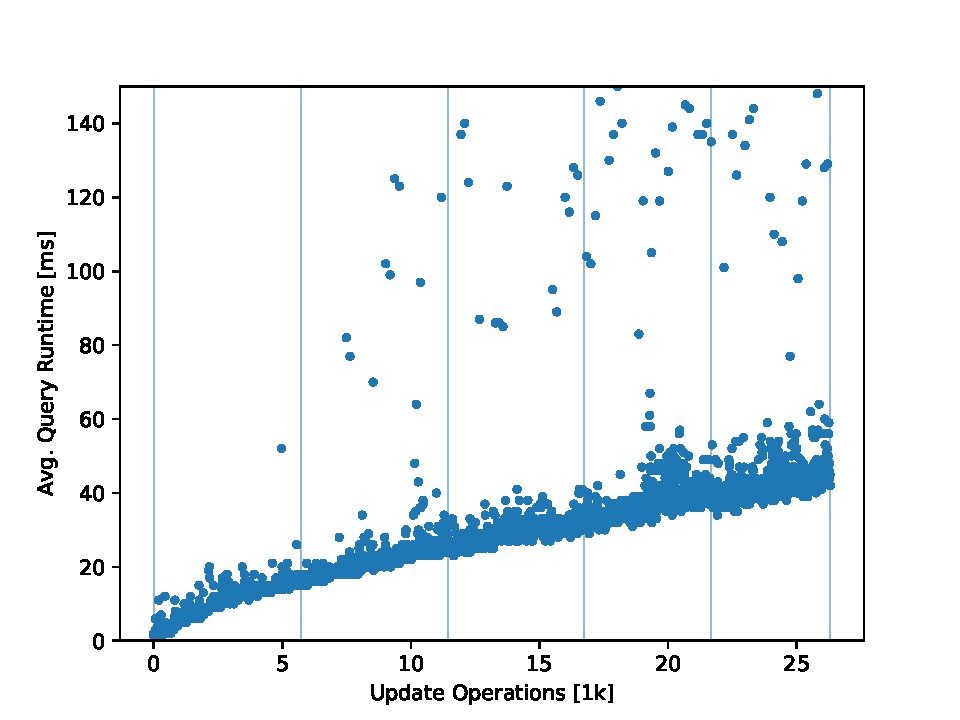
\includegraphics[width=8cm]{query_runtime_synthetic}
    \caption{}
    \label{fig:query_runtime_synthetic}
  \end{subfigure}
  \begin{subfigure}{0.49\linewidth}
    \centering
    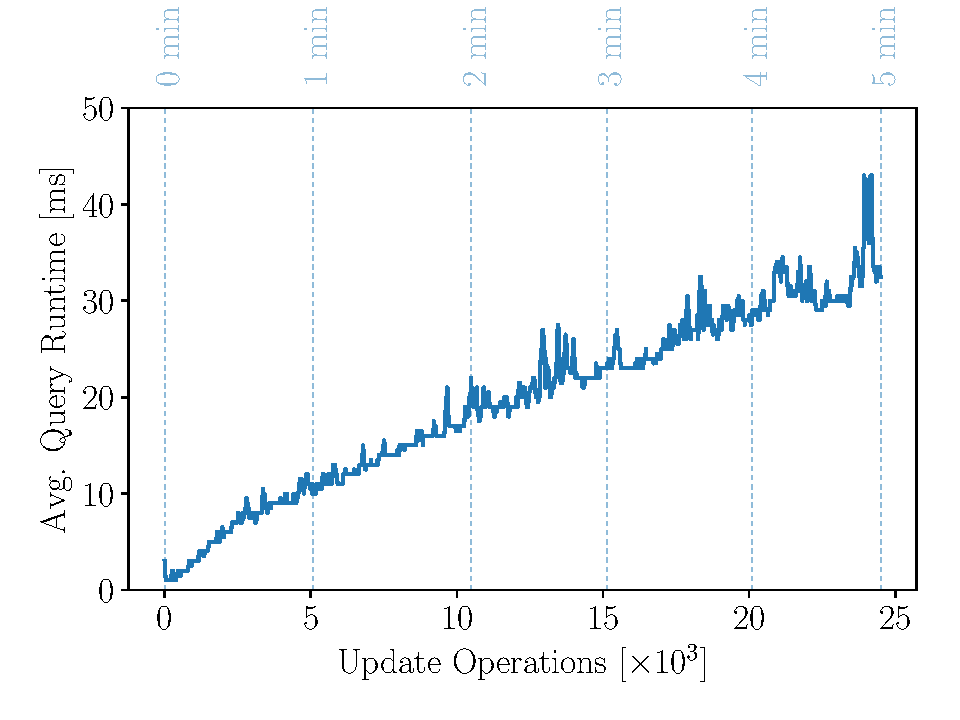
\includegraphics[width=8cm]{query_runtime_real}
    \caption{}
    \label{fig:query_runtime_real}
  \end{subfigure}
  \caption{Query Runtime over time}
  \label{fig:query_runtime}
\end{figure}

\Cref{fig:query_runtime_synthetic,fig:query_runtime_real} show the 
query runtime of the same query as time passes by for the synthetic and
real-world dataset respectively. 
Each point corresponds to the moving median over 10 time points.
We observe a sublinear increase of the runtime from $2 ms$ to $50 ms$
after running the simulation for $5$ minutes ($2.6 \cdot 10^4$ update operations)
on the synthetic dataset and an increase from $2 ms$ to $35 ms$ ($2.5 \cdot
10^4$ update operations) on the real-world dataset. 
% The identical phenomenon is observed
% in \Cref{fig:trav_nodes_synthetic,fig:trav_nodes_real} respectively because
% query runtime depends on the number of nodes traversed during query execution,
% i.e the increase in query runtime is explained by the increase in total
% traversed nodes per query. 

\begin{figure}
  \centering
  \begin{subfigure}{0.49\linewidth}
    \centering
    Synthetic
  \end{subfigure}
  \begin{subfigure}{0.49\linewidth}
    \centering
    Real World
  \end{subfigure}
  \begin{subfigure}{0.49\linewidth}
    \centering
    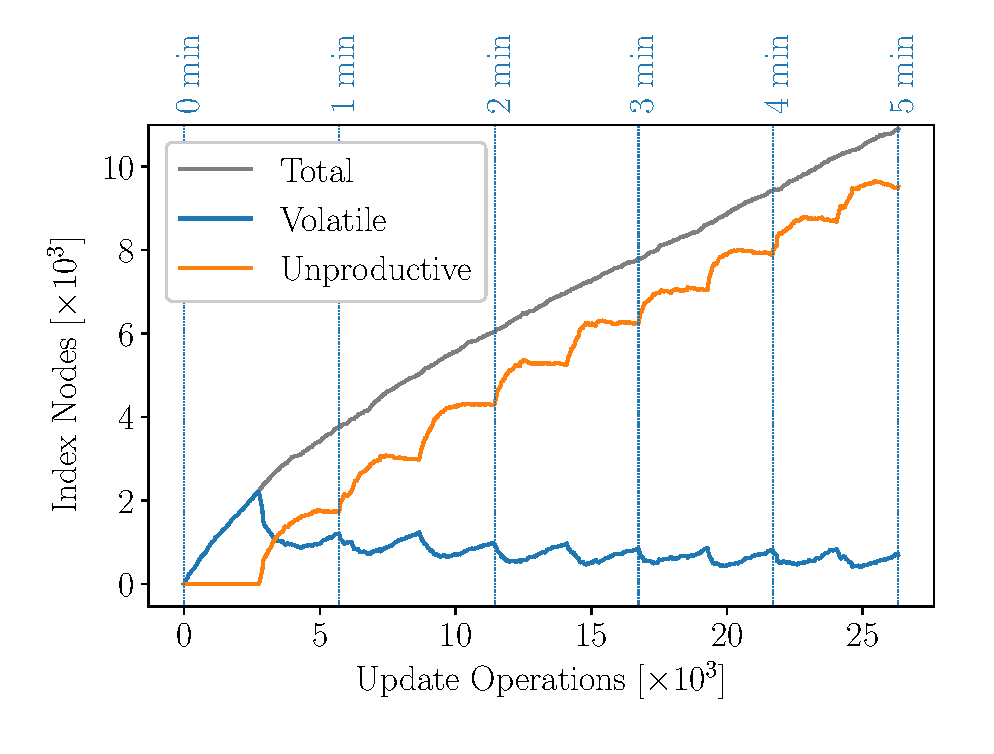
\includegraphics[width=8cm]{trav_nodes_synthetic}
    \caption{}
    \label{fig:trav_nodes_synthetic}
  \end{subfigure}
  \begin{subfigure}{0.49\linewidth}
    \centering
    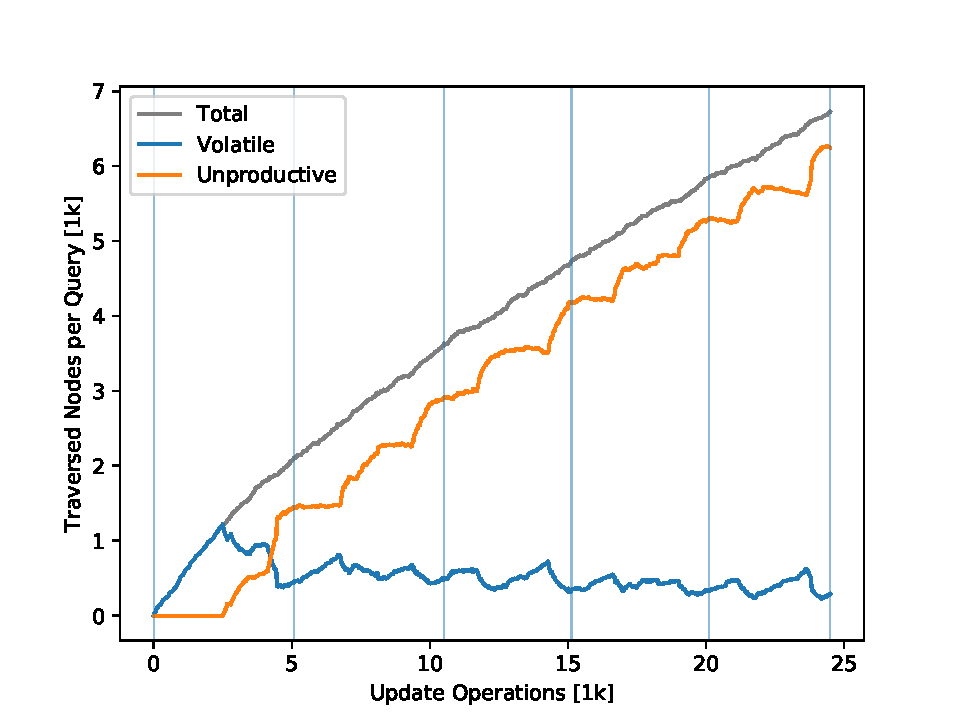
\includegraphics[width=8cm]{trav_nodes_real}
    \caption{}
    \label{fig:trav_nodes_real}
  \end{subfigure}
  \caption{Index composition during Query Execution}
  \label{fig:trav_nodes}
\end{figure}

Next, we present data regarding the type of index nodes traversed during query
execution.
\Cref{fig:trav_nodes_synthetic,fig:trav_nodes_real} depict
the total number of traversed nodes in addition to the number of traversed
volatile and unproductive nodes during query execution for each dataset.

The total number of traversed nodes is increasing sublinearly over time. This
explains the increase in query runtime in
\Cref{fig:query_runtime_synthetic,fig:query_runtime_real}.
As time passes, more and more content nodes are randomly
selected by the CMS workload and their corresponding index nodes become volatile
and, most likely, become
unproductive and are not pruned from the index anymore.
Therefore, the probability of picking a content node with no corresponding index
node (non-indexed)
decreases over time. Since it becomes less and less likely for a non-indexed content node
to be randomly picked by the CMS workload, the rate of growth of total traversed
index nodes decreases over time.

Furthermore, we see the number of volatile nodes descend after the $30$
second mark. We believe it becomes less likely for nodes to become volatile,
as time passes. When a workload randomly picks a node whose index node is
unproductive, the index
node becomes matching but was not added, thus the volatility count of the node
does not increment. In comparison, if the index node would not exist, the created
index node's volatility count would have been incremented. We infer that it is less
likely for an unproductive node to become volatile again than a non-indexed one.
Our experimental evaluation suggests that the number of
unproductive nodes increases over time. Therefore it becomes less likely for any
node to become volatile over time. This explains the decreasing number of volatile nodes.

The sliding window of length $L$ is set to $30$ seconds, therefore we encounter no
unproductive nodes during the first $30$ seconds of the simulation. Once we
reach the $30$ second mark, our queries encounter unproductive nodes.
From that point, we observe a steep increase in traversed unproductive nodes.
After $1$ minute, we observe the traversed nodes being dominated by
unproductive nodes. The rate of growth of traversed unproductive nodes seems to
decrease over time, which can be explained by the same rationale that cause the
decrease of the rate of growth of total index nodes.

Additionally, we observe the functions of the unproductive and volatile index
nodes having cycloids. In \Cref{fig:trav_nodes_synthetic}, each cusp ($30 s, 60 s,
\dots, 300 s$) represents a point in which the workload changes during the
experiment. When the workload changes, we initially see a steep increase in
unproductive nodes. During that phase, more nodes cease to be volatile than
become volatile. Nodes need to reach the threshold in order to become volatile
and few do, since the skew in the workload only picks a subset of
nodes frequently. Before a new workload kicks in, we observe the opposite
phenomenon. More nodes become volatile than cease to be volatile, because many nodes are
on the verge of becoming volatile and therefore need to be picked fewer times to
become volatile in comparison to the time shortly after the workload kicked in. 

Lastly, we also observe the real-world dataset having a more gentle slope over
the synthetic dataset. Since
the real-world dataset has more content nodes, it is less likely for each
content node to be picked by the zipf distribution. Having a smaller chance to be
picked by the workload implies having less volatile and unproductive nodes in
the index.  

\begin{figure}
  \centering
  \begin{subfigure}{0.49\linewidth}
    \centering
    Synthetic
  \end{subfigure}
  \begin{subfigure}{0.49\linewidth}
    \centering
    Real World
  \end{subfigure}
  \begin{subfigure}{0.49\linewidth}
    \centering
    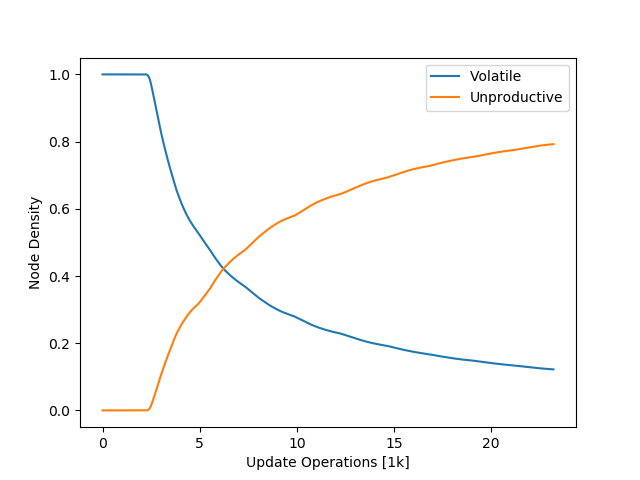
\includegraphics[width=8cm]{trav_node_ratio_synthetic}
    \caption{}
    \label{fig:trav_node_ratio_synthetic}
  \end{subfigure}
  \begin{subfigure}{0.49\linewidth}
    \centering
    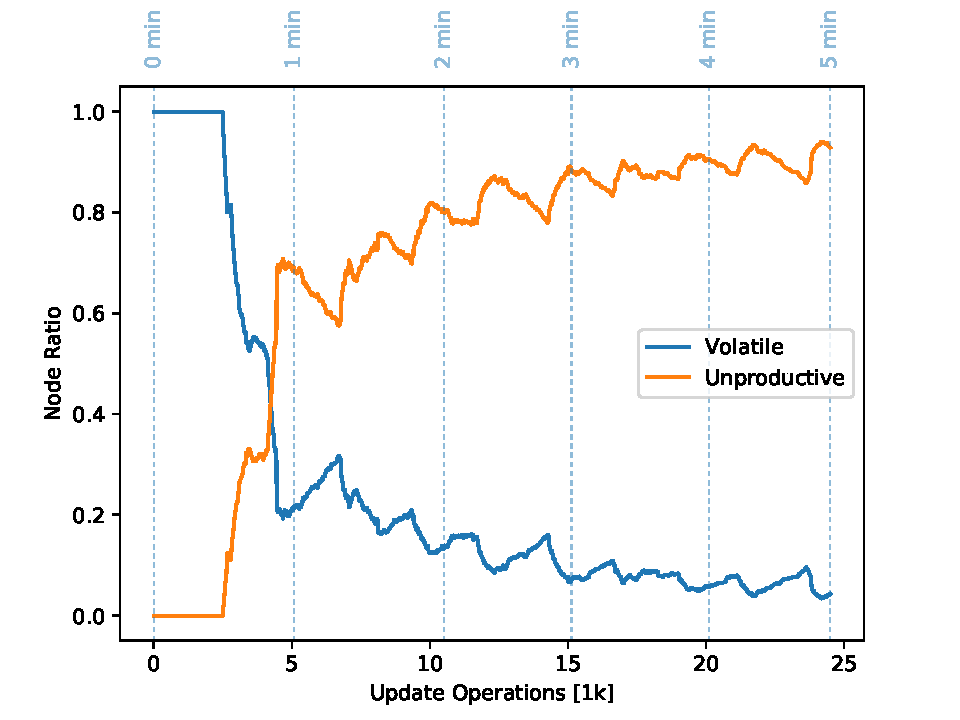
\includegraphics[width=8cm]{trav_node_ratio_real}
    \caption{}
    \label{fig:trav_node_ratio_real}
  \end{subfigure}
  \caption{Node Ratio during Query Execution}
  \label{fig:trav_node_ratio}
\end{figure}

\Crefrange{fig:trav_node_ratio_synthetic}{fig:trav_node_ratio_real}
show the ratio of volatile and unproductive nodes over time and update
operations from our datasets. These figures quantify how strongly unproductive
nodes dominate the traversed nodes. The data shows that unproductive nodes
account for over $80\%$ of the traversed nodes whilst less than $20\%$ are
volatile on the synthetic dataset, $90\%$ and $10\%$ on the real-world dataset,
respectively.

Concluding, the data strongly supports our hypotheses. We see the query runtime
increase as the number of index nodes increases. We also see unproductive nodes
being mostly accountable for the increase in index nodes. 
In the following sections we present two ways dealing with unproductive nodes.

\newpage

\section{Cleaning Unproductive Nodes}

In the previous section, we saw how unproductive nodes slow down query
execution. To prevent unproductive nodes from accumulating in the index, we
clean the index periodically. In the following two subsections, we suggest two
different approaching for dealing with unproductive nodes. We will empirically
investigate their performance in \Cref{sec:experimental-evaluation}.

\subsection{Periodic Garbage Collection (GC)}

First, we propose to clean the index periodically.  Oak has a number of background processes that
maintain the database. We add a background job that periodically executes
garbage collection on Oak.

\Cref{algo:periodic_gc_wapi} takes an index node $n$ as parameter and prunes all
its unproductive descendants. The algorithm traverses
the subtree rooted at $n$. If a descendant $d \in desc(n)$ has no children, is
not matching and not
volatile, it is pruned from the index. The depth-first tree traversal ensures
that the algorithm prunes a child before its parent node. This guarantees that
all unproductive nodes are pruned.

\begin{algorithm}
  \caption{CleanIndexWAPI}
  \DontPrintSemicolon
  \KwData{Index node $n$}
  \For{node $d \in desc(n)$ in DFS}{
    \If{$chd(d) = \emptyset \land \neg matching(d) \land \neg volatile(d)$}{
      delete node $d$\;
    }
  }
  \label{algo:periodic_gc_wapi}
\end{algorithm}

\begin{example}[Periodic GC]
  Consider \Cref{fig:periodic_gc}. Assume index nodes \texttt{/i/pub/now/a/c/e}
  and \texttt{/i/pub/now/a/c} are unproductive in snapshot $G^0$. Oak's
  background thread executes a periodic garbage collection inside transaction
  $T_1$. During $T_1$, the index is traversed in depth-first order.
  The first unproductive node we encounter and prune is
  \texttt{/i/pub/now/a/c/e}. Next, the garbage collector encounters and prunes
  \texttt{/i/pub/now/a/c}. No further unproductive node is left for pruning. We
  see the index after garbage collection in snapshot $G^1$.
\end{example}

\begin{figure}[h]
  \centering

  \begin{large}
    $$ G^0 \xrightarrow{\quad T_1 \quad} G^1$$
  \end{large}

\begin{subfigure}{0.30\textwidth}
  \centering \scriptsize{
    \begin{framed}
      \begin{forest}
        [
        [$\lambda$:$i$
        [$\lambda$:pub
        [$\lambda$:now
        [$\lambda$:$a$
        [$\lambda$:$b$
        [$\lambda$:$d$ \\ pub:now, align=center, base=bottom]
        ]
        [$\lambda$:$c$
        [$\lambda$:$e$]
        ]
        ]
        ]
        ]
        ]
        [$\lambda$:$a$
        [$\lambda$:$b$
        [$\lambda$:$d$ \\ pub:now, align=center, base=bottom]
        ]
        [$\lambda$:$c$
        [$\lambda$:$e$]
        ]
        ]
        ]
      \end{forest}
    \end{framed}
  } \footnotesize{ Snapshot $G^0$ }
\end{subfigure}
\begin{subfigure}{0.30\textwidth}
  \centering \scriptsize{
    \begin{framed}
      \begin{forest}
        [
        [$\lambda$:$i$
        [$\lambda$:pub
        [$\lambda$:now
        [$\lambda$:$a$
        [$\lambda$:$b$
        [$\lambda$:$d$ \\ pub:now, align=center, base=bottom]
        ]
        [,phantom]
        [,phantom]
        ]
        ]
        ]
        ]
        [$\lambda$:$a$
        [$\lambda$:$b$
        [$\lambda$:$d$ \\ pub:now, align=center, base=bottom]
        ]
        [$\lambda$:$c$
        [$\lambda$:$e$]
        ]
        ]
        ]
      \end{forest}
    \end{framed}
  } \footnotesize{ Snapshot $G^1$ }
\end{subfigure}

\vspace{3mm}
\caption*{
  Assume nodes \texttt{/i/pub/now/a/c/e} and \texttt{i/pub/now/a/c} are
  unproductive in snapshot $G^0$. Transaction $T_1$ is executed by the periodic
  garbage collector and committs the resulting snapshot $G^1$.
}
\caption{Garbage collection applied on Oak}
\label{fig:periodic_gc}
\end{figure}

\Cref{fig:java_periodic_gc} shows the java implementation of the periodic
garbage collection task. Calling \texttt{DFS(n)} returns a lazy sequence of nodes
which correspond to a depth-first tree traversal of the subtree rooted at node
\texttt{n}. Next, any node that has children, is matching or volatile is
filtered from the sequence since they are productive. All other nodes are pruned
from the index.

\begin{figure}[h]
\begin{minted}{java}
/**
 * Removes any unproductive descendant of index node n.
 *
 * @param n: index node whose descendants are being cleaned
 */
void cleanIndexWAPI(DocumentNodeState n) {

    /* filter nodes which have children, are matching or volatile */
    for (DocumentNodeState unproductiveNode : filter(
            (DocumentNodeState d) -> d.hasNoChildren() &&
                        !d.getBoolean("match") &&
                        !d.isVolatile()
            ),

            /* DFS tree traversing iterable */
            DFS(n)
    ) {
        unproductiveNode.builder().remove();
    }
}
\end{minted}
  \caption{Java implementation of periodic garbage collection}
  \label{fig:java_periodic_gc}
\end{figure}

\newpage

\subsection{Query Time Pruning (QTP)}

While periodic garbage collection is explicitly executed by Oak in order to
clean unproductive nodes, query time pruning is an approach which clears
unproductive nodes whilst Oak answers queries. By doing so, we benefit by
avoiding the cost of explicitly traversing the index in order to clean it.  

\Cref{algo:query_qtp_wapi} takes a CAS query $Q(k,v,m)$ as an argument, where
$k$ is a property, $v$ a value and $m$ a content node's path. We declare set $r$
and assign it the empty set. $r$ will hold all paths satisfying the CAS query.
We declare node $n$ and assign it the index node corresponding to the content
node with path $m$. Next, we traverse any descendant $d$ of $n$ in depth-first
order. If node $d$ is matching, we add its corresponding content node's path to
$r$ and proceed to the next descendant. If node $d$ is not matching, has no
children and is not volatile, it is deleted from the index. After finishing
traversing the subtree rooted at $n$, we return the result set $r$.

\begin{algorithm}
  \caption{QueryQTP}
  \DontPrintSemicolon
  \KwData{Query $Q(k, v, m)$, where $k$ is a property, $v$ a value and $m$ a
    content node's path.}
  \KwResult{A set of nodes satisfying $Q(k,v,m)$}
  $r \longleftarrow \emptyset$\;
  $n \longleftarrow \texttt{/i/k/v/m}$\;
  \For{node $d \in desc(n)$ in DFS}{
    \uIf{$matching(d)$}{
      $r \longleftarrow r \cup \{ *d \}$\;
    }
    \ElseIf{$chd(d) = \emptyset \land \neg volatile(d)$}{
      delete node $d$
    }
  }
  \Return{r}\;
  \label{algo:query_qtp_wapi}
\end{algorithm}

\begin{example}[QTP]
  Consider \Cref{fig:qtp}. Transaction $T_1$ executes CAS query
  $Q(\texttt{pub},\texttt{now},\texttt{/a/b})$ which queries for all descendants
  of \texttt{/a/b} with ``pub'' set to ``now'' in snapshot $G^0$. Assume the
  query executor uses QTP and nodes \texttt{/i/pub/now/a/b/e} and
  \texttt{/i/pub/now/a/c} are unproductive. The
  query executor traverses all descendants of \texttt{/i/pub/now/a/b} and
  therefore prunes the unproductive index node \texttt{/i/pub/now/a/b/e}. Since
  the other unproductive index nodes are not traversed during query execution,
  they are not pruned and remain in the index unproductive. The resulting
  snapshot $G^1$ is committed by $T_1$ after finishing query execution.
\end{example}


\Cref{fig:java_qtp} shows the java implementation of QTP in Oak. The algorithm
takes a property \texttt{k}, value \texttt{v}, path \texttt{m}, a
\texttt{NodeStore} and returns a lazy sequence of content node paths satisfying
the CAS query $Q(\texttt{k},\texttt{v},\texttt{m})$. We first find index node
$n$. By Calling \texttt{DFS(n)} we get a sequence of nodes representing a
depth-first search in the subtree rooted at $n$. We filter any node that is not
matching from the sequence. If a node has no children, is not matching and is
not volatile, we prune it from the index. next, we take the filtered sequence of
matching index nodes and map them to their corresponding content nodes' path.

\begin{figure}[h]
  \centering
 \begin{large}
    $$ G^0 \xrightarrow{\quad T_1 \quad} G^1$$
  \end{large}

\begin{subfigure}{0.40\textwidth}
  \centering \scriptsize{
    \begin{framed}
      \begin{forest}
        [
        [$\lambda$:$i$
        [$\lambda$:pub
        [$\lambda$:now
        [$\lambda$:$a$
        [$\lambda$:$b$
        [$\lambda$:$d$ \\ pub:now, align=center, base=bottom]
        [$\lambda$:$e$ \\ \vspace{-1mm}, align=center, base=bottom]
        ]
        [$\lambda$:$c$
        [,phantom]
        ]
        ]
        ]
        ]
        ]
        [$\lambda$:$a$
        [$\lambda$:$b$
        [$\lambda$:$d$ \\ pub:now, align=center, base=bottom]
        [$\lambda$:$e$ \\ \vspace{-1mm}, align=center, base=bottom]
        ]
        [$\lambda$:$c$
        [,phantom]
        ]
        ]
        ]
      \end{forest}
    \end{framed}
  } \footnotesize{ Snapshot $G^0$ }
\end{subfigure}
\begin{subfigure}{0.40\textwidth}
  \centering \scriptsize{
    \begin{framed}
      \begin{forest}
        [
        [$\lambda$:$i$
        [$\lambda$:pub
        [$\lambda$:now
        [$\lambda$:$a$
        [$\lambda$:$b$
        [$\lambda$:$d$ \\ pub:now, align=center, base=bottom]
        [,phantom]
        ]
        [$\lambda$:$c$
        [,phantom]
        ]
        ]
        ]
        ]
        ]
        [$\lambda$:$a$
        [$\lambda$:$b$
        [$\lambda$:$d$ \\ pub:now, align=center, base=bottom]
        [$\lambda$:$e$ \\ \vspace{-1mm}, align=center, base=bottom]
        ]
        [$\lambda$:$c$
        [,phantom]
        ]
        ]
        ]
      \end{forest}
    \end{framed}
  } \footnotesize{ Snapshot $G^1$ }
\end{subfigure}

\vspace{3mm}
\caption*{
  Assume nodes \texttt{/i/pub/now/a/b/e} and \texttt{i/pub/now/a/c} are
  unproductive in snapshot $G^0$. Transaction $T_1$ executes CAS query
  $Q(\texttt{pub},\texttt{now},\texttt{/a/b})$ which queries for all descendants
  of \texttt{/a/b} with ``pub'' set to ``now'' and committs the resulting
  snapshot $G^1$. QTP is used during query execution. 
}
 
  \caption{Query Time Pruning applied to Oak}
  \label{fig:qtp}
\end{figure}

\begin{figure}[h]
  \centering
\begin{minted}{java}
/**
 * Answers a CAS Query and prunes traversed unproductive index nodes.
 *
 * @param k: Property
 * @param v: Value
 * @param m: path of content node in which we execute the query
 * @param store: Oak's database interface
 * @returns an iterable with content paths satisfying the CAS query
 */
Iterable<String> QueryQTP(String k, String v, String m, DocumentNodeStore store) {

    /* e.g: /oak:index/pub/:index/now */
    String indexRootPath = concat(OAK_INDEX_PREFIX, k, OAK_INDEX_INTERNAL, v); 

    /* e.g: /oak:index/pub/:index/now/a */
    String targetNodePath = concat(indexRootPath, m);

    DocumentNodeState n = getNode(targetNodePath, store);

    /* map index nodes' path to corresponding content nodes' path */
    return map((DocumentNodeState n) -> relativize(indexRootPath, n.getPath()),

        /* filter non-matching index nodes */
        filter((DocumentNodeState d) -> {
                boolean matching = d.getBoolean("match");

                /* prune if no children, not matching and not volatile */
                if (d.hasNoChildren() &&
                    !matching &&
                    !d.isVolatile()
                ) {
                    d.builder().remove();
                }
                return matching;
            },

            /* DFS tree traversal of descendants of n */
            DFS(n)
    );
}
\end{minted}
  \caption{Java implementation of QTP}
  \label{fig:java_qtp}
\end{figure}

\newpage

\section{Experimental Evaluation}
\label{sec:experimental-evaluation}

\subsection{Goals}

Using the experiment, we wish to learn more about how different parameters
affects the performance of periodic garbage collection and query time pruning.
We initially see how different values of the volatility threshold $\tau$
and sliding window of length $L$ impact unproductive nodes in the index. Next,
we investigate the effects periodicity of garbage collection has in its
algorithms performance. Since the effectiveness of QTP depends on the query
workload, we will investigate how different query workloads affect the overall
performance of QTP. We also conduct an experiment in order to examine how
workload skew impacts the performance of GC and QTP. Finally, we run simulations
in order to see how the update to query ration affects the performance of GC and QTP.

\subsection{Setup}

\subsection{Datasets}

For our experiments we make use of 2 datasets. Each dataset resembles the
content subtree. The \textit{synthetic} dataset is a complete binary tree with
max height 20 and $2^20 \approx 10^6$ nodes. The real-world dataset contains
$1.3 \cdot 10^6$ and is unbalanced. It is taken from an online shop built on top
of Adobe's AEM.

\subsection{Workload}

We paid a lot of attention to the way we simulate a changing workload during the
experiments. The goal was to design a function $f$, which given two integer
arguments, one randomly selected integer $k$ and another representing the
current workload. $f$ returns a new integer representing the picked content node.

We calculate the current workload integer by dividing the time passed since the
experiment started (in milliseconds) by the workload interval, 30 seconds in our
instance. Doing so, we can change the workload every 30 seconds.

It is crucial that $f$ has an an avalanche effect \cite{HF73}. When changing the
workload, we want $f$ to pick completely different content nodes.

We selected a function that takes the two inputs, concatenates them, hashes the
concatenated value and returns a single integer.

\subsection{Experiments}

\subsubsection{Volatility Threshold $\tau$}

Volatility threshold $\tau$ determines after how many insertions/deletions of an index node
it becomes volatile (see \Cref{def:volatile_node}). In this section, we study the impact of
volatility threshold $\tau$ on unproductive nodes and query runtime.

We hypothesize that an increase in $\tau$ yields a decrease to the number of
traversed unproductive nodes during query execution under a CMS workload. If
$\tau$ increases, it is
less likely for a node to become volatile. Having less volatile nodes should
cause a decrease to the number of unproductive nodes and consequently also query
runtime in the CMS workload.

\begin{shaded}
  \begin{itemize}
  \item[$H_3$:] An increase in $\tau$ yields a decrease to WAPI's query runtime
    under a CMS workload. 
  \item[$H_4$:] An increase in $\tau$ yields a decrease to the number of
    traversed unproductive nodes during WAPI's query execution under a CMS workload.
  \end{itemize}
\end{shaded}

We conduct the same experiment under a varying volatility threshold. 
\Cref{fig:query_runtime_taus_synthetic,fig:query_runtime_taus_real} show
thresholds $\tau \in \{1,5,10\}$ affecting query runtime
over update operations. We observe a decrease in query runtime
while increasing threshold $\tau$.
A lower volatility threshold increases the likelihood of a node
becoming volatile. The amount of volatile nodes also affect the number of
unproductive nodes, since volatile nodes eventually stop being frequently
updated and become unproductive. The increase in unproductive nodes in the index
directly affects query runtime because Oak has to traverse these nodes during
query execution.
\Cref{fig:tau_query_runtime_synthetic,fig:tau_query_runtime_real} compare query
runtime over a range of thresholds. The values picked correspond to
the query runtime after $10^4$ update operations.
We observe a power law relationship between threshold $\tau$ and average query
runtime. As explained above, a lower threshold increases the number of volatile
and consequently also the number of unproductive nodes. More unproductive nodes
do increase the query runtime. We believe the power law relationship is
explained by the zipf distribution our workload uses. 

\begin{figure}
  \centering
  \begin{subfigure}{0.49\linewidth}
    \centering
    Synthetic
  \end{subfigure}
  \begin{subfigure}{0.49\linewidth}
    \centering
    Real World
  \end{subfigure}
  \begin{subfigure}{0.49\linewidth}
    \centering
    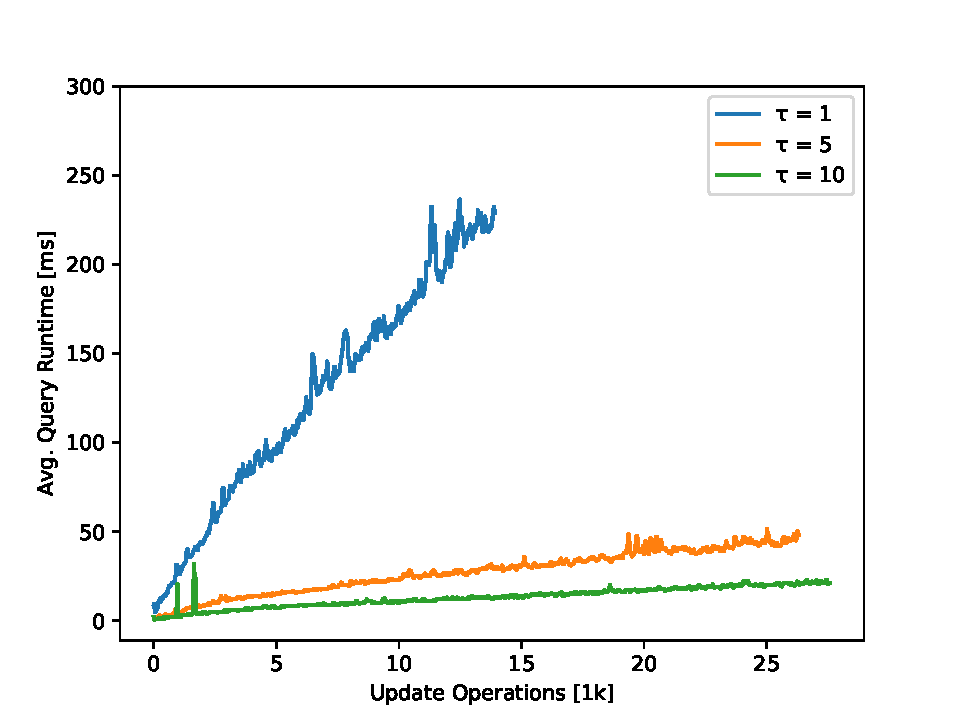
\includegraphics[width=8cm]{query_runtime_taus_synthetic}
    \caption{}
    \label{fig:query_runtime_taus_synthetic}
  \end{subfigure}
  \begin{subfigure}{0.49\linewidth}
    \centering
    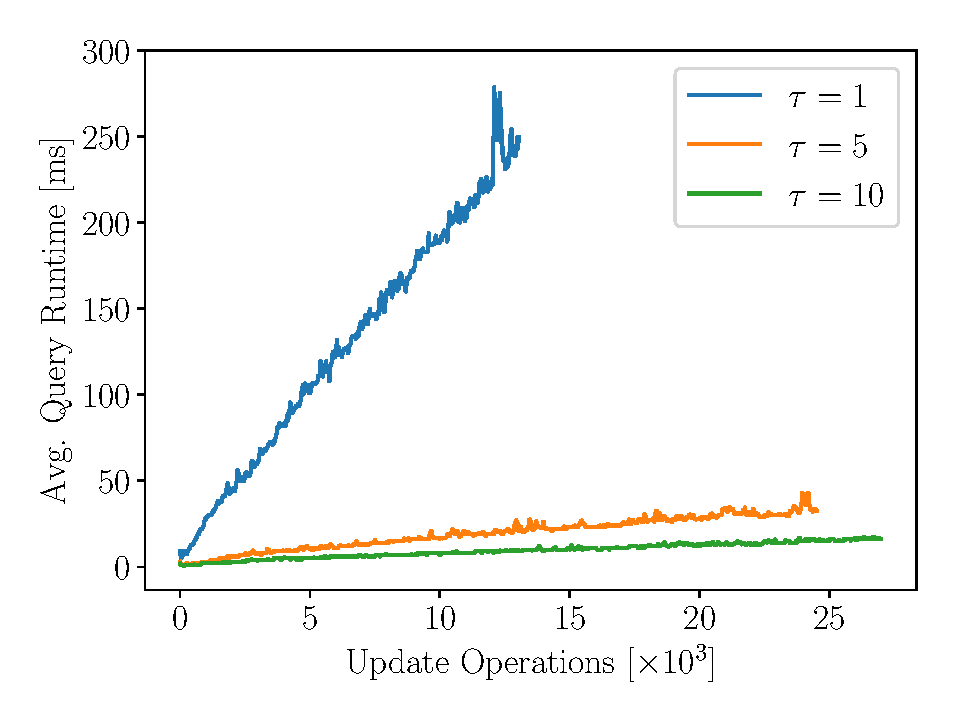
\includegraphics[width=8cm]{query_runtime_taus_real}
    \caption{}
    \label{fig:query_runtime_taus_real}
  \end{subfigure}
  \begin{subfigure}{0.49\linewidth}
    \centering
    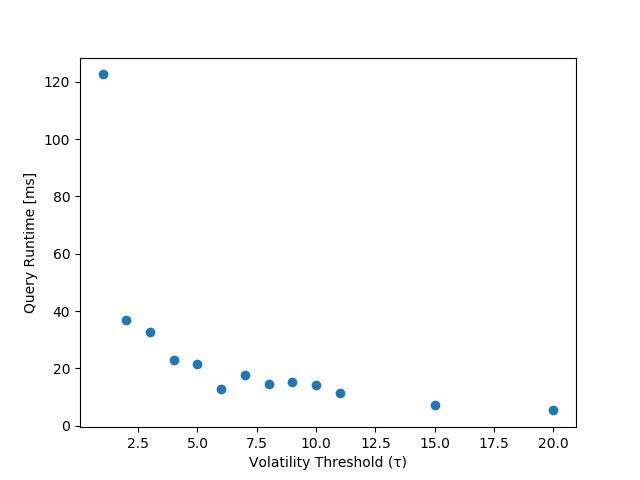
\includegraphics[width=8cm]{tau_query_runtime_synthetic}
    \caption{}
    \label{fig:tau_query_runtime_synthetic}
  \end{subfigure}
  \begin{subfigure}{0.49\linewidth}
    \centering
    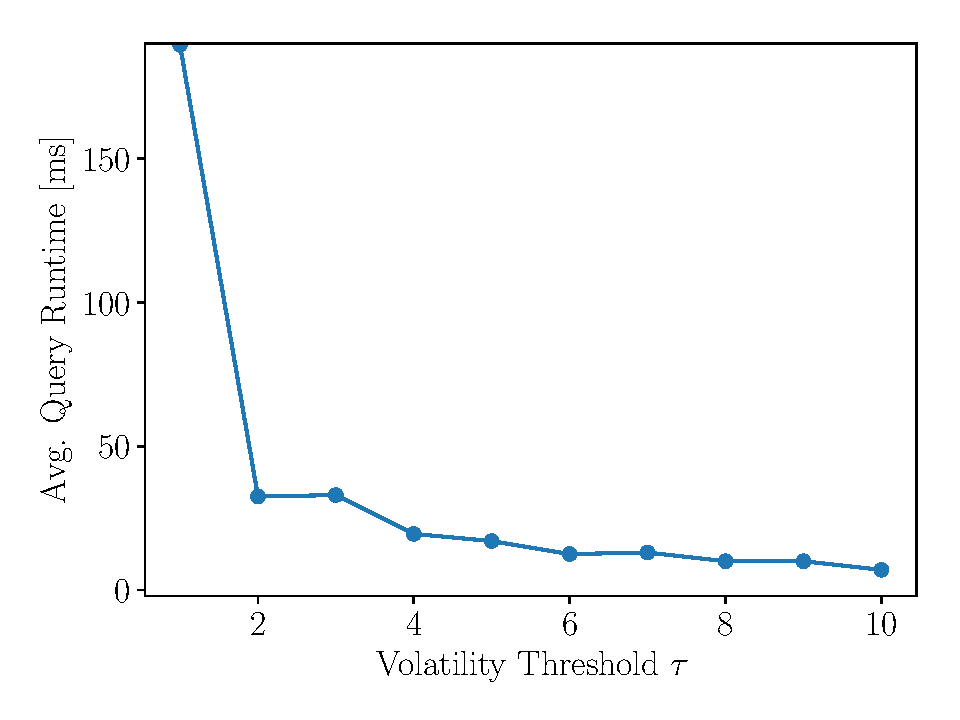
\includegraphics[width=8cm]{tau_query_runtime_real}
    \caption{}
    \label{fig:tau_query_runtime_real}
  \end{subfigure}
\caption{Impact of Volatility Threshold $\tau$ on Query Runtime}
\end{figure}

\Cref{fig:trav_unprod_nodes_taus_synthetic,fig:trav_unprod_nodes_taus_real}
depict thresholds $\tau \in \{1,5,10\}$ affecting the number of unproductive
nodes traversed during query execution over update operations. We observe lower
thresholds $\tau$ yielding in a steeper slope.
\Cref{fig:tau_trav_unprod_nodes_synthetic,fig:tau_trav_unprod_nodes_real} compare the
number of traversed unproductive nodes during query execution over a range of
thresholds. We observe a decrease in unproductive nodes while increasing
threshold $\tau$. As suggested earlier, a lower volatility threshold
increases the amount of volatile nodes in the index. Volatile nodes eventually
cease to be volatile and become unproductive. 

We also see in this figure
the two variables sharing a power law relationship as well. We believe the
workload's zipf skew to be responsible for the power law relationship. We see
the query executor having to traverse $5k$ unproductive index nodes with a
threshold of $\tau = 5$. By increasing the threshold to $\tau = 6$, the average
number of traversed unproductive nodes does not decrease significantly because
of the zipf-distribution's skewness. We believe the decrease to be bigger if the
distribution were less skewed. Having less skew implies more nodes being picked
by the workload.

\begin{figure}
  \centering
  \begin{subfigure}{0.49\linewidth}
    \centering
    Synthetic
  \end{subfigure}
  \begin{subfigure}{0.49\linewidth}
    \centering
    Real World
  \end{subfigure}
  \begin{subfigure}{0.49\linewidth}
    \centering
    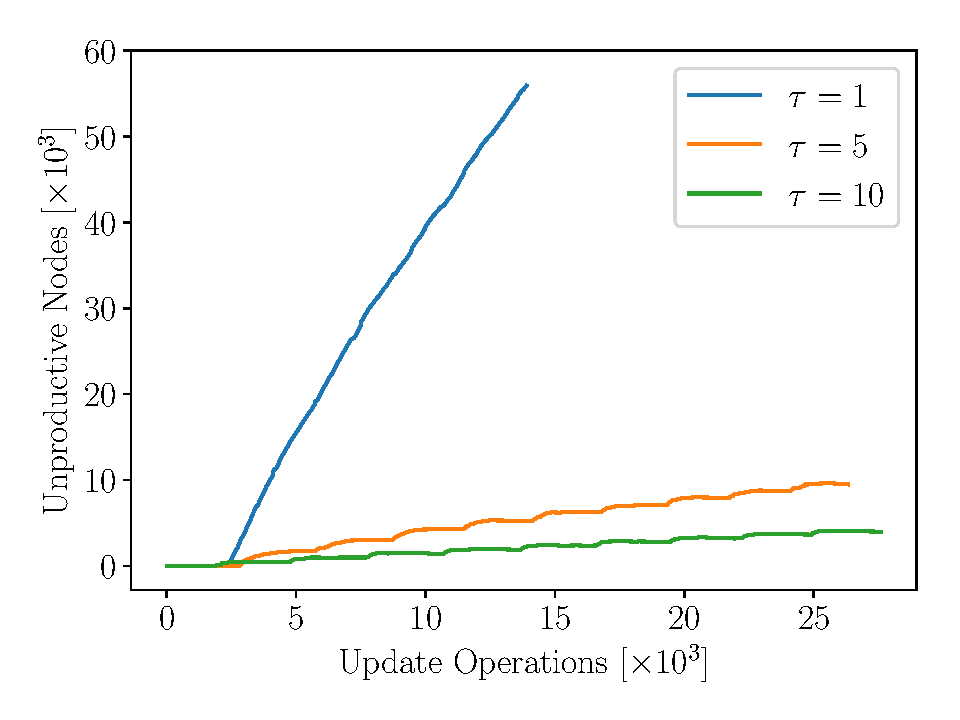
\includegraphics[width=8cm]{trav_unprod_nodes_taus_synthetic}
    \caption{}
    \label{fig:trav_unprod_nodes_taus_synthetic}
  \end{subfigure}
  \begin{subfigure}{0.49\linewidth}
    \centering
    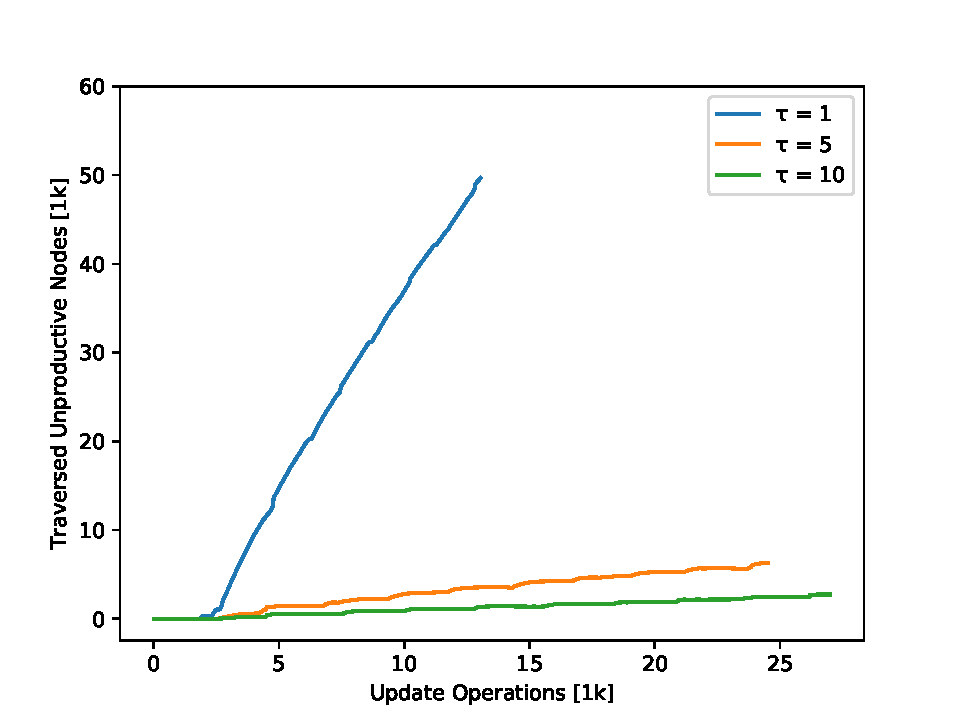
\includegraphics[width=8cm]{trav_unprod_nodes_taus_real}
    \caption{}
    \label{fig:trav_unprod_nodes_taus_real}
  \end{subfigure}
  \begin{subfigure}{0.49\linewidth}
    \centering
    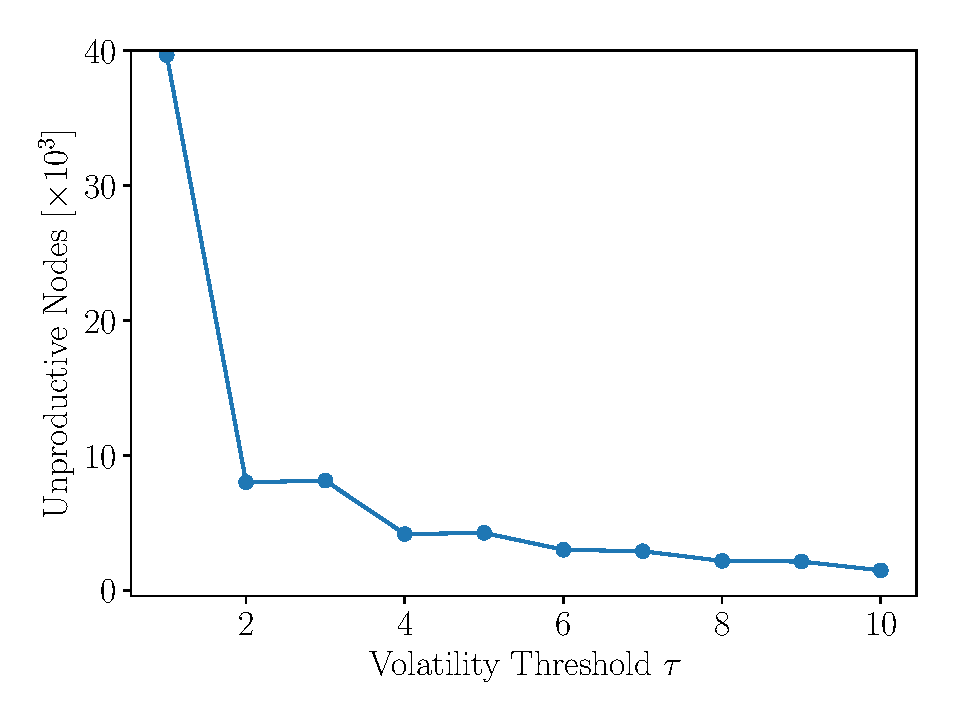
\includegraphics[width=8cm]{tau_unprod_nodes_synthetic}
    \caption{}
    \label{fig:tau_trav_unprod_nodes_synthetic}
  \end{subfigure}
  \begin{subfigure}{0.49\linewidth}
    \centering
    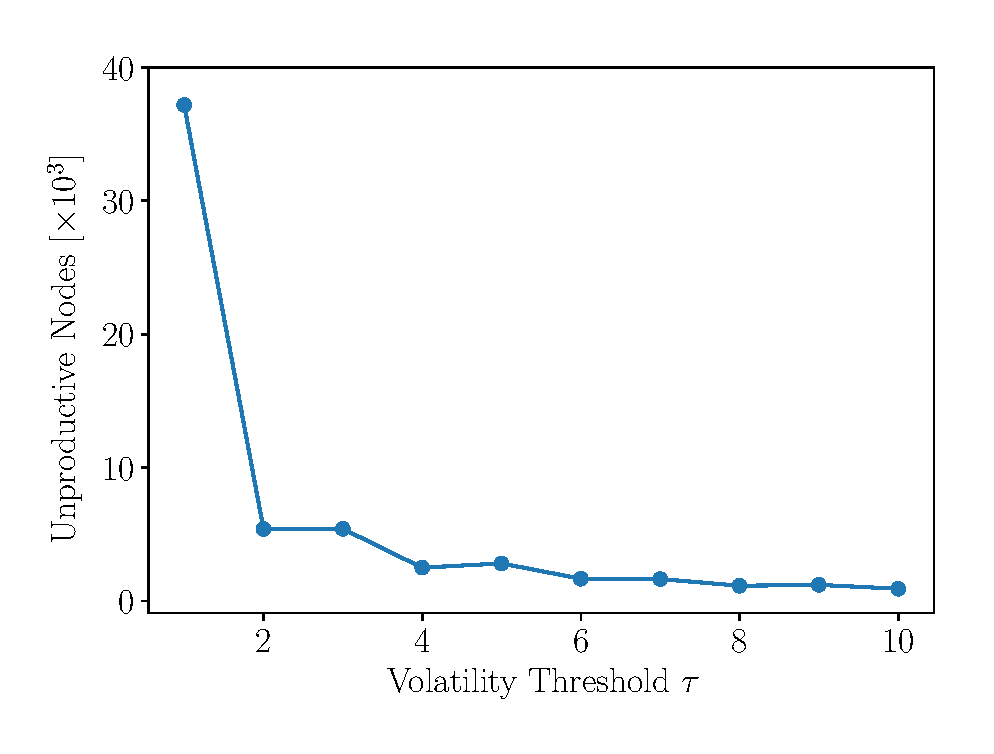
\includegraphics[width=8cm]{tau_unprod_nodes_real}
    \caption{}
    \label{fig:tau_trav_unprod_nodes_real}
  \end{subfigure}
  \caption{Impact of Volatility Threshold $\tau$ on Unproductive Nodes}
\end{figure}

Summarizing, all observations verify hypotheses $H_3$ and $H_4$.
Increasing volatility threshold $\tau$ decreases the number of unproductive
nodes traversed which decreases query runtime. Increasing the volatility
threshold causes less nodes become volatile. Since we create less volatile
nodes, we also reduce the number of unproductive nodes. Less unproductive
nodes yield lower WAPI query runtimes. Another factor affecting the rate of
growth of unproductive nodes is sliding window of length $L$. The following
section addresses the effects of the sliding window.

\subsubsection{Sliding Window of Length $L$}

Sliding window of length $L$ determines the length of the recent workload that WAPI
considers to compute an index node's volatility count. Greater values of $L$
allow WAPI to consider more updates and therefore increase the chances of a node
becoming volatile. In this section, we study
the effect of the sliding window on unproductive nodes and query runtime.

We hypothesize that an increase in $L$ yields an increase to the number of
traversed unproductive nodes during query execution. If $L$ increases, it is
more likely for a node to become volatile, since more updates are considered
towards the volatility count.
Having more volatile nodes should imply an increase in unproductive nodes and
consequently also query runtime in the CMS workload.

\begin{shaded}
  \begin{itemize}
  \item[$H_5$:] An increase in $L$ yields an increase to WAPI's query runtime
    under a CMS workload. 
  \item[$H_6$:] An increase in $L$ should increase the number of unproductive
    nodes WAPI traverses during query execution under a CMS workload.
  \end{itemize}
\end{shaded}

% We conduct our experiment with a varying sliding window length and present our
% observations below.

\Cref{fig:query_runtime_Ls_synthetic,fig:query_runtime_Ls_real} show WAPI's average
query runtime over update operations with sliding window of length $L \in \{10, 20,
30\}$ seconds.
\Cref{fig:L_query_runtime_synthetic,fig:L_query_runtime_real} depict query
runtime with respect to the sliding window length. 
We see queries being executed by a WAPI with a greater sliding
window length to have greater runtimes on average. By increasing the sliding
window, we increase the likelihood of a node becoming volatile. More volatile
nodes result in an increase in unproductive nodes. Since the WAPI has to traverse
more unproductive nodes during query execution, the query runtime increases.

\begin{figure}
  \centering
  \begin{subfigure}{0.49\linewidth}
    \centering
    Synthetic
  \end{subfigure}
  \begin{subfigure}{0.49\linewidth}
    \centering
    Real World
  \end{subfigure}
  \begin{subfigure}{0.49\linewidth}
    \centering
    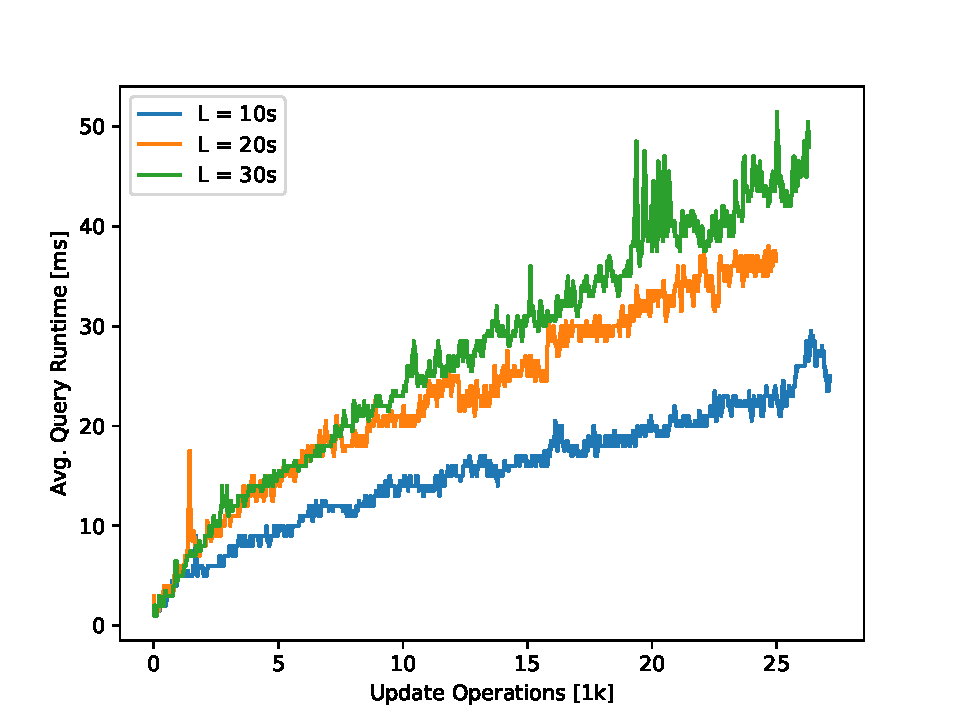
\includegraphics[width=8cm]{query_runtime_Ls_synthetic}
    \caption{}
    \label{fig:query_runtime_Ls_synthetic}
  \end{subfigure}
  \begin{subfigure}{0.49\linewidth}
    \centering
    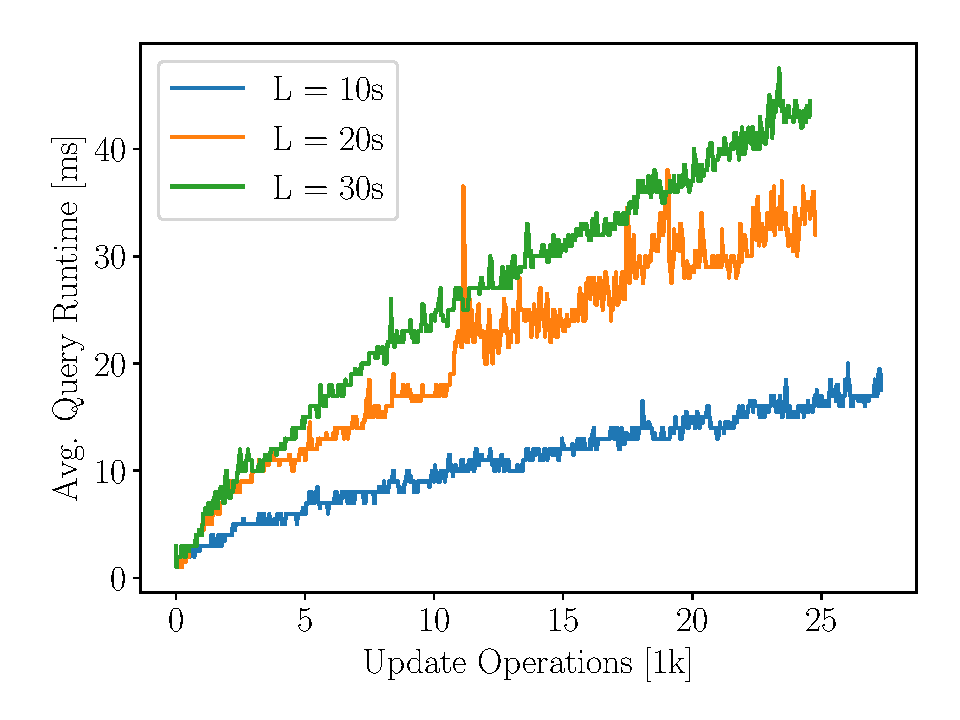
\includegraphics[width=8cm]{query_runtime_Ls_real}
    \caption{}
    \label{fig:query_runtime_Ls_real}
  \end{subfigure}
  \begin{subfigure}{0.49\linewidth}
    \centering
    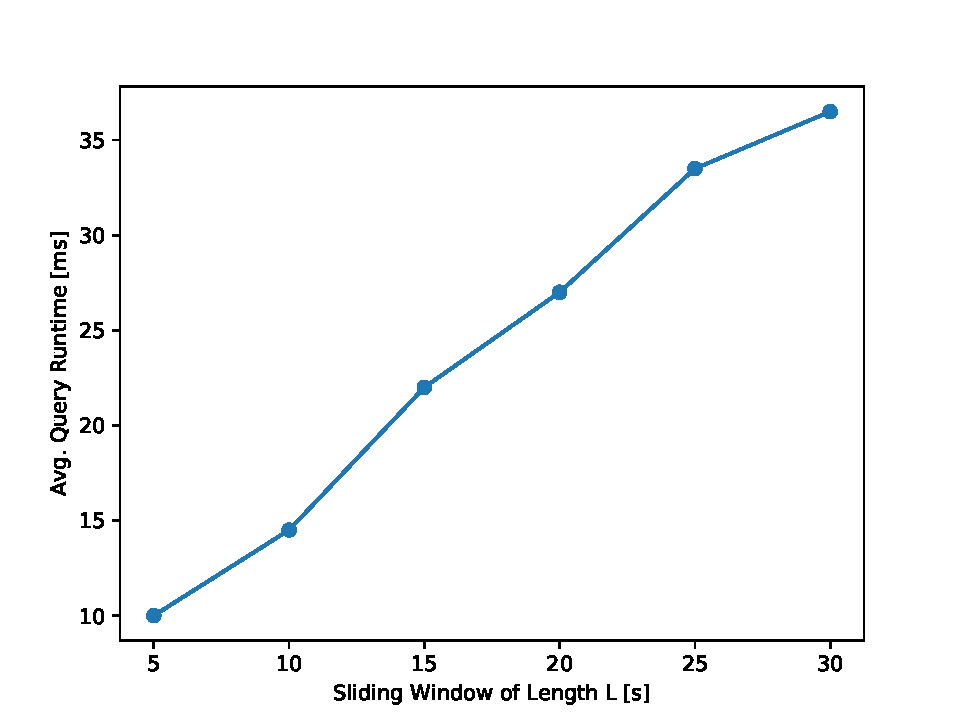
\includegraphics[width=8cm]{L_query_runtime_synthetic}
    \caption{}
    \label{fig:L_query_runtime_synthetic}
  \end{subfigure}
  \begin{subfigure}{0.49\linewidth}
    \centering
    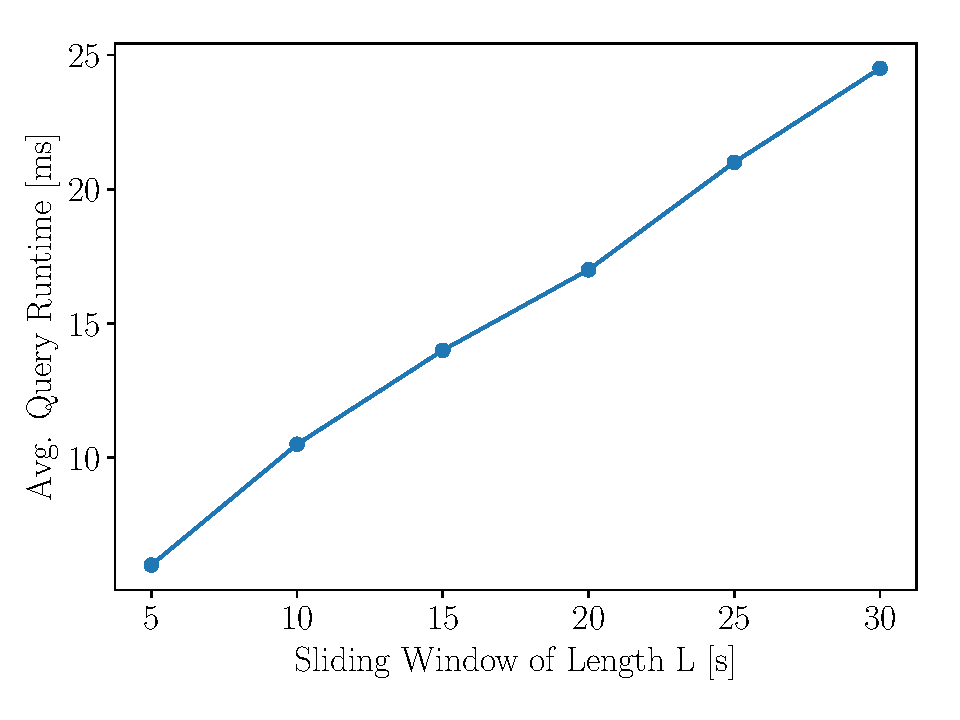
\includegraphics[width=8cm]{L_query_runtime_real}
    \caption{}
    \label{fig:L_query_runtime_real}
  \end{subfigure}
  \caption{Impact of Sliding Window of length $L$ on Query Runtime}
\end{figure}


\Cref{fig:trav_unprod_nodes_Ls_synthetic,fig:trav_unprod_nodes_Ls_real} show the
number of unproductive nodes the WAPI has traversed during query execution. As
expected, we observe greater sliding window lengths to cause an increase to the
rate of growth of unproductive nodes traversed by WAPI during query execution.
More volatile nodes imply an increase in unproductive nodes in the index.

\begin{figure}
  \centering
  \begin{subfigure}{0.49\linewidth}
    \centering
    Synthetic
  \end{subfigure}
  \begin{subfigure}{0.49\linewidth}
    \centering
    Real World
  \end{subfigure}
  \begin{subfigure}{0.49\linewidth}
    \centering
    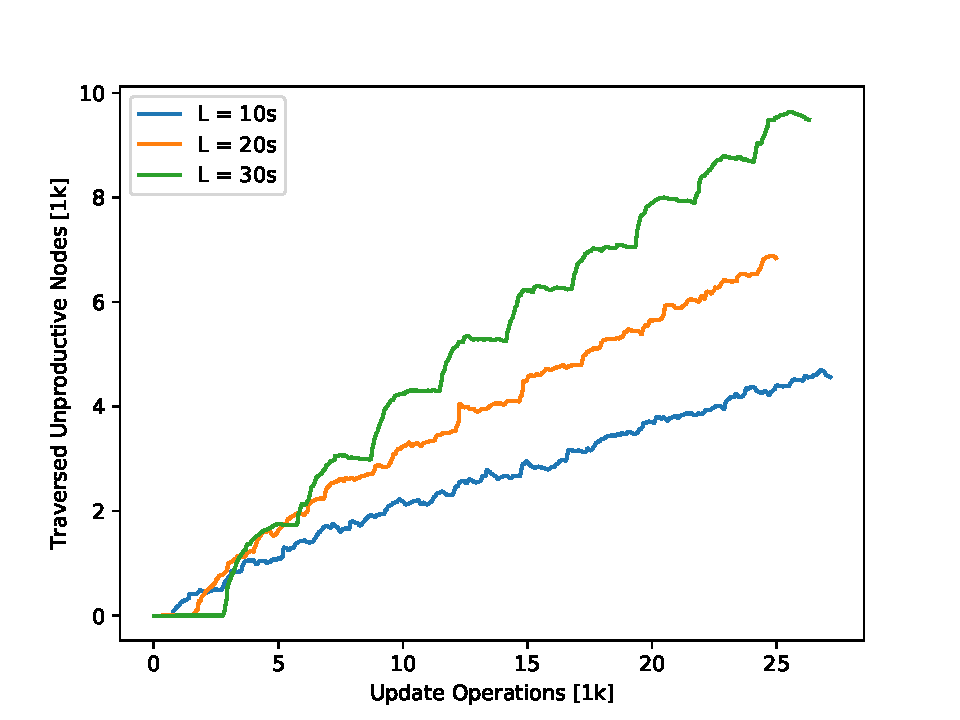
\includegraphics[width=8cm]{trav_unprod_nodes_Ls_synthetic}
    \caption{}
    \label{fig:trav_unprod_nodes_Ls_synthetic}
  \end{subfigure}
  \begin{subfigure}{0.49\linewidth}
    \centering
    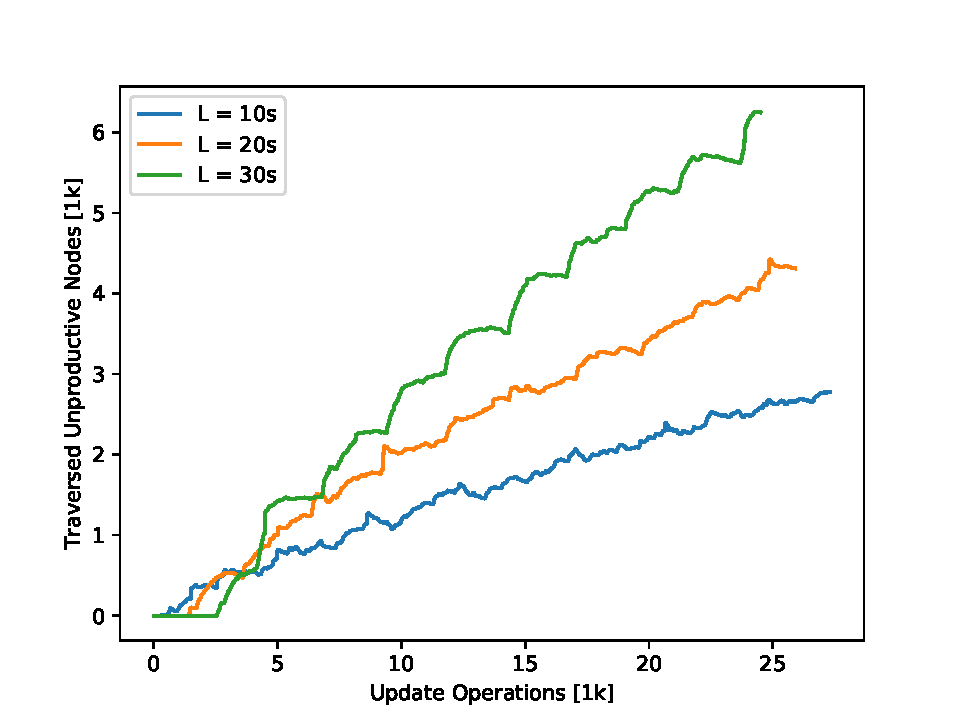
\includegraphics[width=8cm]{trav_unprod_nodes_Ls_real}
    \caption{}
    \label{fig:trav_unprod_nodes_Ls_real}
  \end{subfigure}
  \begin{subfigure}{0.49\linewidth}
    \centering
    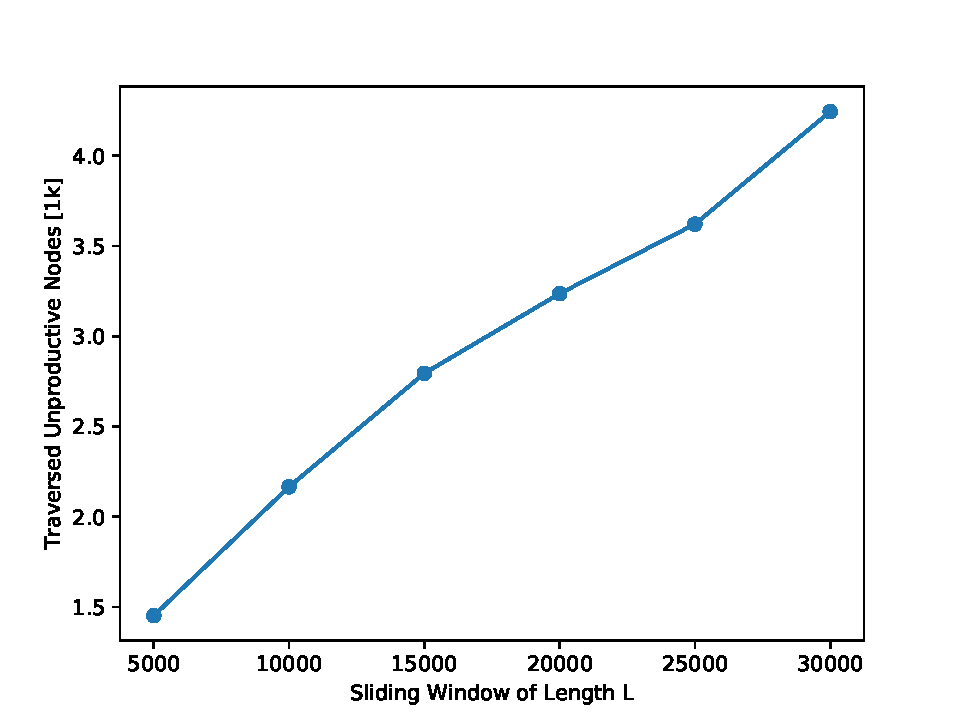
\includegraphics[width=8cm]{L_unprod_nodes_synthetic}
    \caption{}
    \label{fig:L_trav_unprod_nodes_synthetic}
  \end{subfigure}
  \begin{subfigure}{0.49\linewidth}
    \centering
    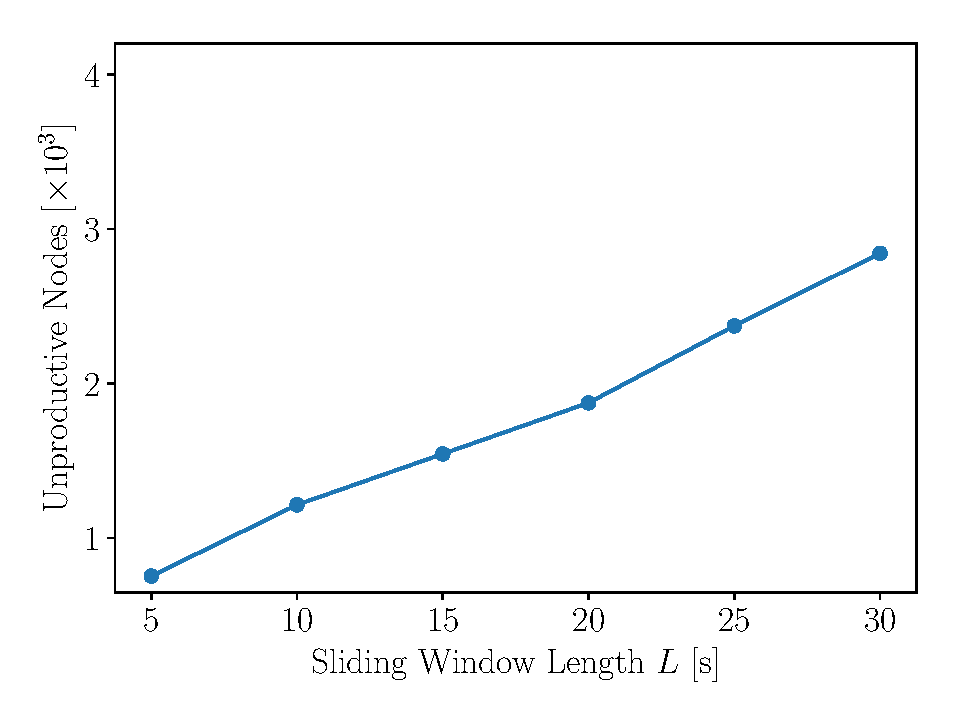
\includegraphics[width=8cm]{L_unprod_nodes_real}
    \caption{}
    \label{fig:L_trav_unprod_nodes_real}
  \end{subfigure}
  \caption{Impact of Sliding Window Length $L$ on Unproductive Nodes}
\end{figure}

Concluding, we see sliding window of length $L$ to be affecting query runtime.
Increasing $L$ does increase the likelihood of an index node become volatile.
More volatile nodes cause an increase in unproductive index nodes. Since the
WAPI has to traverse more index nodes during query execution, its query runtime
increases.

\subsubsection{GC Periodicity}

\subsubsection{QTP Queried Nodes}

\subsubsection{Workload Skew}

\subsubsection{Update to Query ratio}

% In order to empirically evaluate and compare GC and QTP under a changing
% workload, a experiment harness has to be setup.

% datasets

% zipf distribution

% changing Workload

% parameters

\section{Appendix}

\begin{figure}
  \centering
\begin{minted}{java}
/**
 * Returns an iterable which lazily traverses a subtree rooted at root
 * in a depth-first order.
 *
 * @param root: Root node of subtree we apply traversal on
 * @returns: iterable for DFS tree traversal
 */
Iterable<DocumentNodeState> DFS(DocumentNodeState root) {
    return () -> {
        /* Stacks */
        Deque<DocumentNodeState> s1 = new LinkedList();
        Deque<DocumentNodeState> s2 = new LinkedList();
        s1.push(root);
        return new Iterator<DocumentNodeState>() {
            @Override
            public boolean hasNext() {
                return s1.size() > 0 || s2.size() > 0;
            }
            @Override
            public DocumentNodeState next() {
                while (s1.size() > 0 && (
                    s2.size() == 0 ||
                        isAncestor(
                            s2.peek().getPath(),
                            s1.peek().getPath()
                        )
                )) {
                    DocumentNodeState n = s1.pop();
                    s2.push(n);
                    for (ChildNodeEntry child : n.getChildNodeEntries()) {
                        s1.push((DocumentNodeState) child.getNodeState());
                    }
                }
                return s2.pop();
            }          
        };
    };
}
\end{minted}
% \end{verbatim}
  \caption{\texttt{DFS()} implementation}
  \label{fig:java_dfs}
\end{figure}

\begin{figure}
  \centering
% \begin{verbatim}
\begin{minted}{java}
/**
 * Higher order function that applies func to each element of iterable.
 *
 * @param func: The function to apply on each element of iterable
 * @param iterable: The iterable func is applied on
 * @returns: An iterable with the resulting elements of the application
 */
Iterable<R> map(Function<T,R> func, Iterable<T> iterable) {
    return () -> {
        Iterator<T> iterator = iterable.iterator();
        return new Iterator<R>() {
            @Override
            public boolean hasNext() {
                return iterator.hasNext();
            }
            @Override
            public R next() {
                return func.apply(iterator.next());
            }
        };
    };
}
\end{minted}
% \end{verbatim}
  \caption{\texttt{map()} implementation}
  \label{fig:java_map}
\end{figure}

\begin{figure}
  \centering
  % \begin{verbatim}
\begin{minted}{java}
/**
 * Higher order function that removes all elements from an iterable
 * not satisfying the predicate.
 *
 * @param predicate: The predicate that tests elements
 * @param iterable: The iterable whose members are tested against
 * @returns: An iterable with members satisfying the predicate
 */
Iterable<T> filter(Predicate<T> predicate, Iterable<T> iterable) {
    return () -> {
        Iterator<T> iterator = iterable.iterator();
        return new Iterator<T>() {
            private T cur = null;
            @Override
            public boolean hasNext() {
                nextIfNeeded();
                return cur != null; 
            }
            @Override
            public T next() {
                nextIfNeeded();
                T tmp = cur;
                cur = null;
                return tmp;
            }
            @Override
            private void nextIfNeeded() {
                while (cur == null && iterator.hasNext()) {
                    T candidate = iterator.next();
                    if (predicate.test(candidate)) {
                        cur = candidate;
                    }
                }
            }
        };
    };
}
\end{minted}
% \end{verbatim}
  \caption{\texttt{filter()} implementation}
  \label{fig:java_filter}
\end{figure}

\newpage

\bibliographystyle{abbrv}
\bibliography{thesis}

\end{document}
